\documentclass[12pt,a4paper,english,twoside,openright]{report}
\usepackage{parskip}

%\usepackage[left=2.5cm,right=2.5cm,top=2cm]{geometry}
\usepackage[includeheadfoot, inner=3.5cm, outer=3.5cm]{geometry}
\setlength{\headheight}{15pt}

\usepackage{emptypage}
\usepackage{fancyhdr}
\pagestyle{fancy}
\fancyhf{}
\fancyhead[LE,RO]{\thepage}
\renewcommand{\sectionmark}[1]{ \markright{\thesection\ #1}{} }
\fancyhead[RE,LO]{\rightmark}
%\fancyfoot[CE,CO]{\thepage}
%\fancyfoot[LE,RO]{\thepage}

\usepackage{fontspec}
\defaultfontfeatures{
  Extension = .otf,
  Path = fonts/,
  UprightFont = *-Regular,
  BoldFont = *-Bold,
  ItalicFont = *-Italic,
  BoldItalicFont = *-BoldItalic,
}
\setmainfont[Scale = 0.9]{Charter}
\newfontfamily\headingfont{Charter}
% \setmainfont[Scale = 0.8]{Merriweather}
% \newfontfamily\headingfont{Sansita}
\setmonofont[Scale = 0.85]{SourceCodePro}

\usepackage{titlesec}
\titleformat{\chapter}[display]
  {\headingfont\bfseries}{\LARGE\chaptertitlename\ \thechapter}{5pt}{\Huge}
\titleformat*{\section}{\LARGE\headingfont\bfseries\itshape}
\titleformat*{\subsection}{\Large\headingfont\itshape}
\titleformat*{\subsubsection}{\large\headingfont}


\usepackage{float}
\floatstyle{boxed}
\restylefloat{figure}

\usepackage{amsfonts}
\usepackage{amsmath}
\usepackage{subdepth}

\DeclareMathOperator{\shap}{vts}
\DeclareMathOperator{\cfs}{cfs}
\DeclareMathOperator{\fold}{fold}
\DeclareMathOperator{\csh}{csh}
\DeclareMathOperator{\opt}{opt}

\usepackage{xcolor}
%\usepackage[gray]{xcolor}
\definecolor{mygreen}{RGB}{0, 100, 0}
\definecolor{mygray}{RGB}{245, 245, 245}

\usepackage{tikz}
\usetikzlibrary{graphs}
\usetikzlibrary{graphdrawing}
\usetikzlibrary{arrows, automata}
\usetikzlibrary{backgrounds}
\usegdlibrary{layered}


% Double brackets and braces for shapes:
% \vect{ expr }
% \recd{ expr }
% \tupl{ expr }

\usepackage{stmaryrd}

\newcommand\vect[1]{\llbracket #1 \rrbracket}
\newcommand\tupl[1]{\langle\kern-0.25em\langle #1 \rangle\kern-0.25em\rangle}

\usepackage{xparse}

% Based on:
% https://tex.stackexchange.com/questions/252648/left-right-double-curly-brace-blackboard-bold-symbol
\NewDocumentCommand{\recd}{sO{}m}{%
  \IfBooleanTF{#1}
    {\recdext{#3}}
    {\recdx[#2]{#3}}%
}

\NewDocumentCommand{\recdext}{m}{%
  \sbox0{%
    \mathsurround=0pt % just for safety
    $\left\{\vphantom{#1}\right.\kern-\nulldelimiterspace$%
  }%
  \sbox2{\{}%
  \left\{\kern-.7\wd0\left\{#1\right\}\kern-.7\wd0\right\}%
}

\NewDocumentCommand{\recdx}{om}{%
  \sbox0{\mathsurround=0pt$#1\{$}%
  \sbox2{\{}%
    \mathopen{#1\{\kern-.7\wd0 #1\{}
    #2
    \mathclose{#1\}\kern-.7\wd0 #1\}}
}


\usepackage{minted}
\newmintinline[ir]{rust}{}
\newmintedfile[rustfile]{rust}{}
% \rustfile[firstline=2,lastline=7,gobble=4]{rustcode/examples/references.rs}

\usepackage{enumerate}
\usepackage{multicol}
\usepackage{dirtytalk}
\usepackage{pdfpages}
\usepackage{relsize}

\newcommand\icode[1]{\texttt{\textbf{#1}}}

\newcommand\morestuff{\textcolor{red}{ More stuff here... }}
\newcommand\placeholder[1]{\textcolor{red}{Placeholder: #1}}

\catcode`\‹ =\active
\def‹#1›{\texttt{\textbf{\detokenize{#1}}}}

\catcode`\« =\active
\def«#1»{\emph{\detokenize{#1}}}
\def\fsharpdata{\emph{F\# Data}}
\def\cpp{{C\raisebox{.07em}{\smaller\kern-.07em+\kern-.09em+}}}

\title{Rust types from JSON samples}
%\subtitle{A macro based approach to type providers in Rust}
\author{Erik Vesteraas}
\date{}

\usepackage[
  pdftitle={Rust types from JSON samples},
  pdfauthor={Erik Vesteraas},
  unicode=true,
  colorlinks=true,
  linkcolor=black,
  urlcolor=mygreen,
  citecolor=mygreen
]{hyperref}
\urlstyle{same}

\usepackage[
  backend=biber,
  %style=authoryear,
  maxbibnames=6,
  isbn=false,
  %url=false,
  doi=false,
  defernumbers=true
]{biblatex}
\addbibresource{refs.bib}
\setlength\bibitemsep{\baselineskip}

\begin{document}

\pagenumbering{roman}
\includepdf[pages={-}]{forside.pdf}
\setcounter{page}{5}

\tableofcontents

\listoflistings
\listoffigures

\cleardoublepage

%!TEX root = ../main.tex

\vspace*{2cm}

\begin{center}

\section*{\hfil Reading notes \hfil}

The most recent version of this document can be found at \url{http://vestera.as/thesis/}. The \LaTeX\ source can be found at \url{https://github.com/evestera/thesis}. If you come across any typos while reading this, or have any feedback in general, feel free to open an issue at \url{https://github.com/evestera/thesis/issues} or send me an email at \href{mailto:erik@vestera.as}{\nolinkurl{erik@vestera.as}}.

\subsection*{\hfil Typographic conventions \hfil}

\begin{tabular}{ r l }
Clickable link & \href{https://www.rust-lang.org/}{Rust Programming Language} \\
Inline code & ‹true || false› \\
Project or library name & «json_typegen» \\
\end{tabular}

\end{center}


\cleardoublepage

%!TEX root = ../main.tex

\vspace*{2cm}
\thispagestyle{plain}

\begin{center}

\phantomsection
\addcontentsline{toc}{section}{Abstract}

\section*{\hfil Abstract \hfil}

\end{center}

When programmers access external data in a statically typed programming language, they are often faced with a dilemma between convenient and type-safe access to the data.

In the programming language F\#, a concept called type providers has been proposed as a solution to this problem by having compiler support for libraries with the capability to generate types at compile time.

This thesis presents «json_typegen», a project which aims to show the feasibility of similar solutions in the Rust programming language. The project uses compile-time metaprogramming along with alternative interfaces to the same code generation implementation to achieve convenient, type-safe access to data in the JSON data format. While JSON is chosen as the format for the presented library, the approach also applies to other data formats and sources.


\cleardoublepage

\pagenumbering{arabic}

%!TEX root = ../main.tex

\chapter{Introduction}
\label{chap:introduction}

\begin{picture}(0,0)
\put(190,50){\hbox{
\includegraphics[width=4.2cm, angle=-5, trim=4 4 4 4, clip]{ferris/book}}}
\end{picture}
\vspace{-1cm}

When programmers write programs that access external data in a statically typed programming language, they are often faced with a dilemma between convenience and type-safe access to the data they wish to use. For type-safe access, significant boiler-plate code or types must usually be written.

In the programming language F\#, a concept called type providers has been proposed as a solution to this problem by having compiler support for libraries with the capability to generate custom types that reflect the external data, at compile time.

This thesis presents «json_typegen», a project which aims to show the feasibility of similar solutions in the Rust programming language. The project uses compile-time metaprogramming along with alternative interfaces to the same code generation implementation to achieve convenient, type-safe access to data in the JSON data format. While the presented project provides support for JSON specifically, the approach, and much of the code used by «json_typegen» can also ber used for other data formats and sources.

In this chapter we will look at the background for the «json_typegen» project.

First, in section~\ref{sec:rust-intro}, we will look at the Rust programming language. Then, in section~\ref{sec:json}, we will look at the JSON data interchange format, and the challenges associated with accessing data in JSON from statically typed programming languages, and Rust in particular. Finally, in section~\ref{sec:type-providers} we will look at how these challenges have been attempted solved with type providers in the programming language F\#.

In chapter~\ref{chap:project-presentation}, the project and its interfaces is presented in detail. And in chapter~\ref{chap:code-generation} we will look at how the code inference and code generation used in the project works.

\section{The Rust programming language}
\label{sec:rust-intro}

The project presented in the thesis, «json_typegen», creates types for programs written in the Rust programming language, and is itself written in Rust. The Rust programming language is a modern, open source programming language with C-like surface syntax. It is a statically typed language with type inference, with a focus on memory safety and zero-cost abstractions.

Rust does not use a garbage collector and the core library can be used without access to heap allocation. This allows Rust to be used for what is often referred to as \say{systems programming}, e.g. for writing drivers, operating systems and code for microcontrollers. Spaces which has so far been occupied mainly by C and \cpp\footnote{There are \emph{some} other languages that can be said to compete in this area, like Ada, Objective-C and D. I won't go into the details of how these languages compare to Rust, but for various reasons \cpp\ is the main competitor and point of comparison for most use cases.}. Rust tries to combine the low-level control of these languages with modern syntax and an advanced type system that statically prevents whole classes of memory safety issues\cite{the-rust-language}.

While the basic syntax of Rust can be said to be C-like it also has a lot of functionality and syntax reminiscent of functional languages and in particular languages of the ML-family. Features such as closures, pattern matching and monadic error handling are available and a significant part of idiomatic Rust code.

What follows is a very basic introduction to the parts of Rust we need to talk about in this thesis. Many of Rusts more advanced language features are not necessary to understand the basic concepts of this thesis, and are as such not explained here. For more details on the language features of Rust, see \href{https://doc.rust-lang.org/book/}{the Rust book}\footnote{\url{https://doc.rust-lang.org/book/}}.

\subsection{Structs}

\begin{listing}[ht!]
\begin{minted}{rust}
struct Person {
    name: String,
    age: i64,
}
\end{minted}
\caption{A basic Rust struct}
\label{lst:struct}
\end{listing}

The primary language construct for complex types in Rust are structs. A struct declaration, as shown in Listing~\ref{lst:struct}, is a sequence of field names, along with their types. Structs are product types and are analogous to records in some languages. Rust does not have classes or objects, and is not object oriented in the classical sense. In other words is there no inheritance between structs, and polymorphism in Rust is instead supported by other language features, such as enumerated types, and traits.

\subsection{Enums}

\begin{listing}[ht!]
\begin{minted}{rust}
enum Option<T> {
    None,
    Some(T),
}
\end{minted}
\caption{The enumerated type ‹Option› in Rust}
\label{lst:enum}
\end{listing}

An enum in Rust is a data type that is one alternative from a number of variants, i.e. an enumerated type, sum type or union. A declaration of an enum, as seen in Listing~\ref{lst:enum} is given as a list of variant names, used as constructors. Each variant can optionally carry some associated data.

Rust supports pattern matching on enum types and verifies that any match is exhaustive.

\subsection{Traits}
\label{sec:traits}

A trait specifies methods that a type needs to provide to implement the trait. On a superficial level, traits in Rust are similar to interfaces in languages like Java, and type classes in Haskell.

\begin{listing}[ht!]
\begin{minted}{rust}
trait Clone {
    fn clone(&self) -> Self;
}

#[derive(Debug)]
struct Bag {
    label: String
}

impl Clone for Bag {
    fn clone(&self) -> Self {
        Bag {
          label: self.label.clone()
        }
    }
}
\end{minted}
\caption{The Rust trait ‹Clone› and examples of implementation}
\label{lst:trait}
\end{listing}

Listing~\ref{lst:trait} shows the trait ‹Clone›, which is a slightly simplified version of a trait in the Rust standard library. The trait defines the function ‹clone›, which takes as its argument a reference to an instance of the type implementing the trait -- ‹&self› -- and returns a new copy of the same type -- ‹Self›.

The listing also shows a struct, ‹Bag›, which implements two traits. ‹Bag› implements the trait ‹Clone› with an ‹impl Clone› block, providing an implementation of the required function.

In addition to the manual implementation of ‹Clone›, the trait ‹Debug›, is \say{derived}, i.e. automatically implemented by the compiler, using an annotation, \mbox{\icode{\#[derive(Debug)]}}. The code for this automatic implementation is included with the compiler, but it is also possible to write libraries that can derive custom traits. Deriving a trait usually requires that the constituent types also implements the trait. E.g. to derive ‹Clone› for ‹Ty› you need to be able to clone all parts of ‹Ty›.

\subsection{Macros}
\label{sec:macros}

A macro system is in short a language feature that allows a programmer to write code that does source-to-source transformations, also known as metaprogramming. In Rust there are two categories of macros: declarative macros and procedural macros, which are both expanded at compile time.

\begin{listing}[ht!]
\textbf{Macro declaration:}
\begin{minted}{rust}
macro_rules! double {
    ($e: expr) => ({
        let temp = $e;
        temp + temp
    })
}
\end{minted}
\vspace{5mm}

\textbf{Macro usage:}
\begin{minted}{rust}
let ten = double!(2 + 3);
\end{minted}
\caption{A simple declarative macro in Rust}
\label{lst:macro-rules}
\end{listing}

Declarative macros in Rust are also known as \say{macros by example} or \say{pattern-based macros}. These are syntactic, hygienic macros that with a syntax similar to pattern matching, match input patterns to expanded source code. Listing~\ref{lst:macro-rules} show declaration and usage of a very basic declarative macro. The macro ‹double› has a single rule transforming a single expression to a block expression. A macro can have multiple rules and each pattern can be a combination of tokens and metavariables.

Procedural macros are macros where the expansion is done by running a procedure rather than by evaluating rules. To create a procedural macro in Rust you create a library that exposes a function that takes a ‹TokenStream› as input and outputs a ‹TokenStream›. Since this library and function can use arbitrary Rust code to generate its output, it can do things that are outside the scope of the normal compiler. Examples of things there are already procedural macro libraries for are:

\begin{itemize}
  \item Generating a type-safe DSL (at compile time) for communicating with an SQL database, by inspecting said database.\cite{diesel}
  \item Compiling graphics shaders at Rust compile time.\cite{vulkano}
\end{itemize}

% Possible expansions here:
% - Current state of macros in Rust. Past, future.

\subsection{Cargo}

Cargo is the package manager and build tool for the Rust ecosystem. While not a part of the Rust programming language itself, it is provided alongside the compiler in every normal installation. Cargo makes it easy to create new packages -- \say{crates} in Rust terminology -- build them, and manage other crates as dependencies.

While users of some programming languages may be accustomed to build systems with good dependency management this is not the case for users of the traditional systems level languages, C and \cpp. The part of «json_typegen» that comes closest to working like a type provider is a library the user adds a dependency to their project. Thanks to the availability of Cargo, this is an almost insignificant barrier for potential users of the project.

For a perspective on the difference in the development experience it is useful to look at how the experience of going from nothing to a minimal project with a dependency is in Rust and \cpp.

In appendix~\ref{app:cargo-cpp-comparison} I have included a comparison of setting up a project using both Cargo and what I currently consider to be the best alternative in the \cpp\ ecosystem. While the specifics are not important, suffice to say that setting up a project and adding dependencies in Rust using Cargo is significantly easier and more easily reproducible than the equivalent scenario using \cpp.

% Possible expansions here:
% - Example of Cargo.toml and cargo commands
% - Sentence about crates.io

\section{JSON}
\label{sec:json}

JSON is a text-based data format for structured data. It is very commonly used as a data interchange format in modern HTTP-based architectures. JSON was originally based on a subset of the JavaScript programming language, but is designed to be language-independent and is now used in the interaction between applications written in practically all programming languages.

\begin{listing}[ht!]
\begin{align*}
\textit{value} ::=  &\ \textit{object} \mid \textit{array} \mid \textit{number} \mid \textit{string} \mid ‹true› \mid ‹false› \mid ‹null› \\
\textit{object} ::=  &\ \icode{\{}\ [\ \textit{string}\ ‹:›\ \textit{value}\ \text{*}(\ ‹,›\ \textit{string}\ ‹:›\ \textit{value}\ )\ ]\ \icode{\}} \\
\textit{array} ::= &\ ‹[›\ [\ \textit{value}\ \text{*}(\ ‹,›\ \textit{value}\ )\ ]\ ‹]› \\
\textit{number} ::= &\ [\ ‹-›\ ]\ \textit{int}\ [\ \textit{frac}\ ]\ [\ \textit{exp}\ ]\ \\
\textit{string} ::= &\ ‹"›\ \text{*}\textit{char}\ ‹"›
\end{align*}
\caption[The JSON grammar]{The JSON grammar from RFC 7159. It is somewhat simplified as the actual specification is very precise. See the full specification for the exact definitions of \textit{int}, \textit{frac}, \textit{exp} and \textit{char}.}
\label{lst:json-grammar}
\end{listing}

The format as described by the two official JSON specifications -- IETF RFC 7159\cite{RFC7159} and ECMA 404\cite{ECMA404} -- is intended to be very simple to write and to parse. As can be seen from the grammar in Listing~\ref{lst:json-grammar} a JSON value can only be an object, array, number or string, or one of the literals ‹true›, ‹false› and ‹null›. In addition, there is no way to define new types, references or to specify external resources or definitions.
% contrast simplicity to XML?

A JSON object is a collection of mappings from keys (that are JSON strings) to JSON values. As this closely corresponds to what is usually referred to as a map or a dictionary in most programming languages, the term object may seem like a bit of a misnomer here, arising from JSONs background as a subset of JavaScript. Whether or not the fields of an object are ordered is explicitly unspecified by RFC 1759, but \say{Implementations whose behavior does not depend on member ordering will be interoperable in the sense that they will not be affected by these differences.}\cite[6]{RFC7159}

A JSON array is an ordered collection of JSON values. It is worth noting that JSON places no restriction on the types of the values of the array, and as such, it can sometimes be a heterogeneous collection.

\begin{listing}[ht!]
\begin{minted}{json}
{
  "name": "Bob",
  "age": 24,
  "phoneNumbers": [
    {
      "areaCode": 456,
      "number": 80931
    }
  ]
}
\end{minted}
\caption{An example JSON object}
\label{lst:json1}
\end{listing}

Listing~\ref{lst:json1} shows a basic example of a JSON object. Since JSON objects and arrays can themselves contain objects and arrays, data serialized as JSON can be arbitrarily deeply nested, but as mentioned JSON itself has no support for any kind of references, so there is no possibility of loops or infinite types.

In RFC 7159 it is stated that \say{the representation of numbers is similar to that used in most programming languages.} However, there are some very significant differences to the most normal number types in most programming languages. A number in JSON can be arbitrarily large, and arbitrarily precise. The only actual rule for a number to be valid JSON is that it satisfies the grammar given in the specifications. As this shows, while the specifications are quite simple, this simplicity leads to some complications and pitfalls.

A JSON string resembles string literals in many programming languages, with characters and escape sequences, like \icode{{\textbackslash}n} or \icode{{\textbackslash}u000a}, enclosed in quotation marks. As seen from the grammar, strings serve double duty in JSON as both object keys and general values. This means that many possible JSON keys can be quite challenging to map to valid identifiers in a programming language. It is for example perfectly valid to have an object with the keys ‹""›, ‹" "› and ‹"µ"›.

% Everything is "nullable"

\subsection{Reading JSON in dynamically typed languages}

\begin{listing}[ht!]
\begin{minted}{js}
var parsed = JSON.parse(jsonString);
console.log(parsed.phoneNumbers[0].areaCode);
\end{minted}
\caption{Printing the first areaCode in JavaScript}
\label{lst:readjsonjs}
\end{listing}

\begin{listing}[ht!]
\begin{minted}{python}
parsed = json.loads(jsonString)
print(parsed["phoneNumbers"][0]["areaCode"])
\end{minted}
\caption{Printing the first areaCode in Python}
\label{lst:readjsonpy}
\end{listing}

In dynamically typed programming languages reading data from deserialized JSON is relatively straightforward, as seen in Listings~\ref{lst:readjsonjs} and~\ref{lst:readjsonpy}, showing parsing and reading in JavaScript and Python\footnote{It is also possible in Python to get the JSON deserialized into such forms that its syntax become more like the direct field access of JavaScript, but the code shown uses the default behaviour.} respectively. The code in these Listings can, however, fail at runtime with exceptions or errors if the deserialized data does not match expectations, e.g. if the field ‹"phoneNumbers"› is missing, or contains a number instead of an array. So in many real world use cases the code will be a bit more complex, to deal with such problems without crashing.

\subsection{Reading JSON in statically typed languages}

In statically typed programming languages reading data from deserialized JSON often requires a bit more effort. There are several possible (and relatively common) approaches.

For my examples I will use Rust, but first I need to introduce «Serde»:

\subsubsection{Serde}
\label{sec:serde}

«Serde»\cite{serde} is a Rust framework for serialization and deserialization. The core of the framework is independent of the source/target data format, and the input/output of specific data formats is provided by separate crates.

«Serde» works by providing two traits, ‹Serialize› and ‹Deserialize›, that Rust types can implement. The core library has already implemented these traits for the most common data types like ‹i64›, ‹String›, ‹Vec› and ‹HashMap›. In addition, the crate «serde_derive» provides code for deriving ‹Serialize› and ‹Deserialize› for custom -- i.e. your own -- types.

Once a Rust type implements the necessary trait, data can be converted with the various format specific crates, that provide implementations for one or both of the traits «Serializer» and «Deserializer». «serde_json»\cite{serdejson} provides implementations of these types for JSON. It also provides some other functionality that is useful for working with JSON.

\subsubsection{Catchall types}

\begin{listing}[ht!]
\begin{minted}{rust}
enum Value {
    Null,
    Bool(bool),
    Number(Number),
    String(String),
    Array(Vec<Value>),
    Object(Map<String, Value>),
}
\end{minted}
\caption{An enumerated type in Rust for JSON values}
\label{lst:valueenum}
\end{listing}

Listing~\ref{lst:valueenum} shows the Rust type ‹Value› from the library «serde_json». Any legal JSON can be encoded by this type. Similar types can be created in most programming languages. However, working with such types in a type-safe manner can be both tedious and error-prone. The code in Listing~\ref{lst:readjsonrs1} does approximately the same thing as the code in Listings~\ref{lst:readjsonjs} and~\ref{lst:readjsonpy}, using pattern matching. While the code is type-safe and will not fail at runtime, it is not particularly convenient.

\begin{listing}[ht!]
\begin{minted}{rust}
let parsed: Value = serde_json::from_str(json_str)?;

if let Some(array) = parsed.get("phoneNumbers") {
    if let Some(obj) = array.get(0) {
        if let Some(num) = obj.get("areaCode") {
            println!("{}", num);
        }
    }
}
\end{minted}
\caption{Printing the first areaCode in Rust using pattern matching}
\label{lst:readjsonrs1}
\end{listing}

% if let Some(num) = parsed.get("phoneNumbers")
%                          .and_then(|v| v.get(0))
%                          .and_then(|v| v.get("areaCode")) {
%     println!("{}", num);
% }

\subsubsection{Stringly typed code}

One way to make the catchall types easier to work with is to create helpers that essentially skips individual checking of each field access. Listing~\ref{lst:readjsonrs2} shows two alternative ways to read from the parsed data.

\begin{listing}[ht!]
\begin{minted}{rust}
let parsed: Value = serde_json::from_str(json_str)?;

println!("{}", parsed["phoneNumbers"][0]["areaCode"]);

if let Some(num) = parsed.pointer("/phoneNumbers/0/areaCode") {
    println!("{}", num);
}
\end{minted}
\caption{Printing the first areaCode in Rust using indexing expressions and JSON pointers}
\label{lst:readjsonrs2}
\end{listing}

The first way shows how it is possible to use indexing syntax -- ‹container[index]› -- with the ‹Value› type, due to the fact that it implements the ‹Index› trait. In other words, very similarly to the syntax one would use with e.g. the default Python solution. While index expressions in Rust \emph{can} panic, the shown expression will actually not do so, as the ‹Value› implementation of the ‹Index› trait instead returns ‹Value::Null› if indexing fails. This does, however, conflate when indexing fails and when the data contains an actual ‹Null› value.

The second approach shown instead uses a string, which encodes a path\footnote{The path is encoded as a JSON Pointer. We will come back to JSON Pointers in more detail in section~\ref{sec:json-pointers}.}, to combine multiple ‹get()› calls into a single function call. This call returns an ‹Option› to distinguish between ‹Null› values and lookup failure, but is otherwise quite similar.

Neither of these approaches, nor the first approach with the individual ‹get()› calls actually gives us a number in the form of an integer, though. What we actually get is\footnote{Assuming the input was the string in Listing~\ref{lst:json1}.} a ‹Value::Number(Number { ... })› which means that if we wanted to do something else than just printing it, our code would still have some unwrapping to do. And with all this, if we misspell a field, we may not even know that the code failed at runtime because of a typo and not some problem with the data.

\subsubsection{Custom types}

What we actually want are custom types, that accurately reflects the actual data. This way, any mismatches between our assumptions and the actual structure of the data is revealed at the time of JSON parsing, and any misspelling of field names is discovered at program compile time.

\begin{listing}[ht!]
\begin{minted}{rust}
#[derive(Deserialize)]
struct Person {
    name: String,
    age: i64,
    phoneNumbers: Vec<PhoneNumber>,
}

#[derive(Deserialize)]
struct PhoneNumber {
    areaCode: i64,
    number: i64,
}

let parsed: Person = serde_json::from_str(json_str)?;

println!("{}", parsed.phoneNumbers[0].areaCode);
\end{minted}
\caption{Printing the first areaCode in Rust using custom types}
\label{lst:readjsonrs3}
\end{listing}

Listing~\ref{lst:readjsonrs3} shows an example of using such custom data types with the «serde» framework. However, even for this small example this approach required 9 significant lines of code for the types. And with real-world data sources, actual JSON data can be significantly larger and more complex. So while custom types are preferable once written, actually writing them can often be a significant hurdle.

\section{Type providers}
\label{sec:type-providers}

Solving the problem of convenient, type-safe access to external resources is of course something that has been thought about before this thesis. F\# is an open source, functional programming language for the Common Language Runtime. Like Rust it is statically typed, and draws inspiration from the ML-family of languages. In version 3.0 of F\# a concept called \say{type providers} was introduced.

As the name suggests the type provider \say{provides} the necessary custom types to the compiler, letting the programmer access the resource without having to spell out the type information manually.

\begin{listing}[ht!]
\begin{minted}{fsharp}
open FSharp.Data

type Simple = JsonProvider<""" { "name":"John", "age":94 } """>

[<EntryPoint>]
let main argv =
    let simple = Simple.Parse(""" { "name":"Jane", "age":4 } """)
    printfn "%s %d" simple.Name simple.Age
    // prints "Jane 4"
    0
\end{minted}
\caption{Minimal example of the use of a type provider in F\#}
\label{lst:fsharpsample}
\end{listing}

Listing~\ref{lst:fsharpsample} shows an example of a type provider, ‹JsonProvider›, in use. The type provider is given a static parameter, in this case a string of JSON. A type is generated from this sample at compile time, and the type is then used to parse another instance, with the same structure, at runtime. The parsed object is then available to be used in a type-safe manner, just like any other instance of a custom type.

To reiterate: the expression ‹JsonProvider<...>› is evaluated at compile time and provides a type to the compiler. This lets the compiler know the type of, and type check, expressions like ‹simple.Age›, even though the type, or even the existence, of the field ‹Age› is not visible anywhere in the actual F\# code. This is somewhat reminiscent of how type inference lets the compiler lets the compiler know the type of a variable like ‹name› in an expression like ‹let name = "Bob"›, even if the type is not visible in code.

The particular type provider shown, ‹JsonProvider›, comes from the library \fsharpdata\cite{fsharpdata}, which has type providers for multiple formats, and the example is adapted from its documentation\footnote{\url{http://fsharp.github.io/FSharp.Data/library/JsonProvider.html}}. Both the sample string and the string providing the instance could have been replaced by paths to either local or remote resources:

\begin{minted}{fsharp}
type Simple = JsonProvider<"http://example.com/person.json">
type Simple = JsonProvider<"samples/person.json">
\end{minted}

The compiler also provides functionality that makes it easy for implementors of editors to provide autocomplete and similar functionality for types generated by type providers. Thus, when writing code that talks to a JSON based API, it is often possible to just point the type provider to an endpoint or a sample from some documentation, and get the types one needs to start working. Possibly even without looking at the JSON, and instead using autocomplete to explore the data.

\subsection{Type providers from an implementation standpoint}

So what \emph{is} a type provider? How do they work? From an implementation standpoint, support for type providers can be boiled down to two features:

\begin{itemize}
  \item Compile-time metaprogramming with access to side effects\footnote{The paper \emph{Dependent Type Providers}\cite{dependent-type-providers}, which shows the use of dependent types in the Idris programming language to create type providers, shows that \say{compile-time metaprogramming with access to side effects} could possibly be replaced with \say{type creation abilities with side effects}.}, with the expressiveness of a full programming language.
  \item Support for thunks, i.e. lazy or delayed evaluation, of at least parts of the abstract syntax tree, and letting such thunks be made by compile-time metaprogramming.
\end{itemize}

Additionally, for a type provider to make sense, the language has to be statically typed. In a dynamically typed language, the types are associated with the runtime instances of values, so providing extra type information before runtime does not provide much benefit. Since type providers can create a large number of types it is also beneficial if the language has type inference so the actual names of the sub-types are less significant.

As we looked at in section~\ref{sec:macros}, Rust does have compile-time metaprogramming with the flexibility of a full programming language, in the form of procedural macros. It is also a statically typed language with type inference. Rust does however not have any ability for procedural macros to let parts of the generated code be created lazily.

In F\# type provider implementations it is possible to add type members as thunks, which are then only evaluated as required by the compiler. This makes it possible for type providers to provide access to data which whose type spaces would otherwise be too large to create custom types for. Just like lazy evaluation makes infinite lists possible, and practical, in languages like Haskell, thunks as parts of the generated types makes arbitrary large or infinite type hierarchies possible, and practical, in F\#.

\begin{figure}[ht!]
\begin{center}
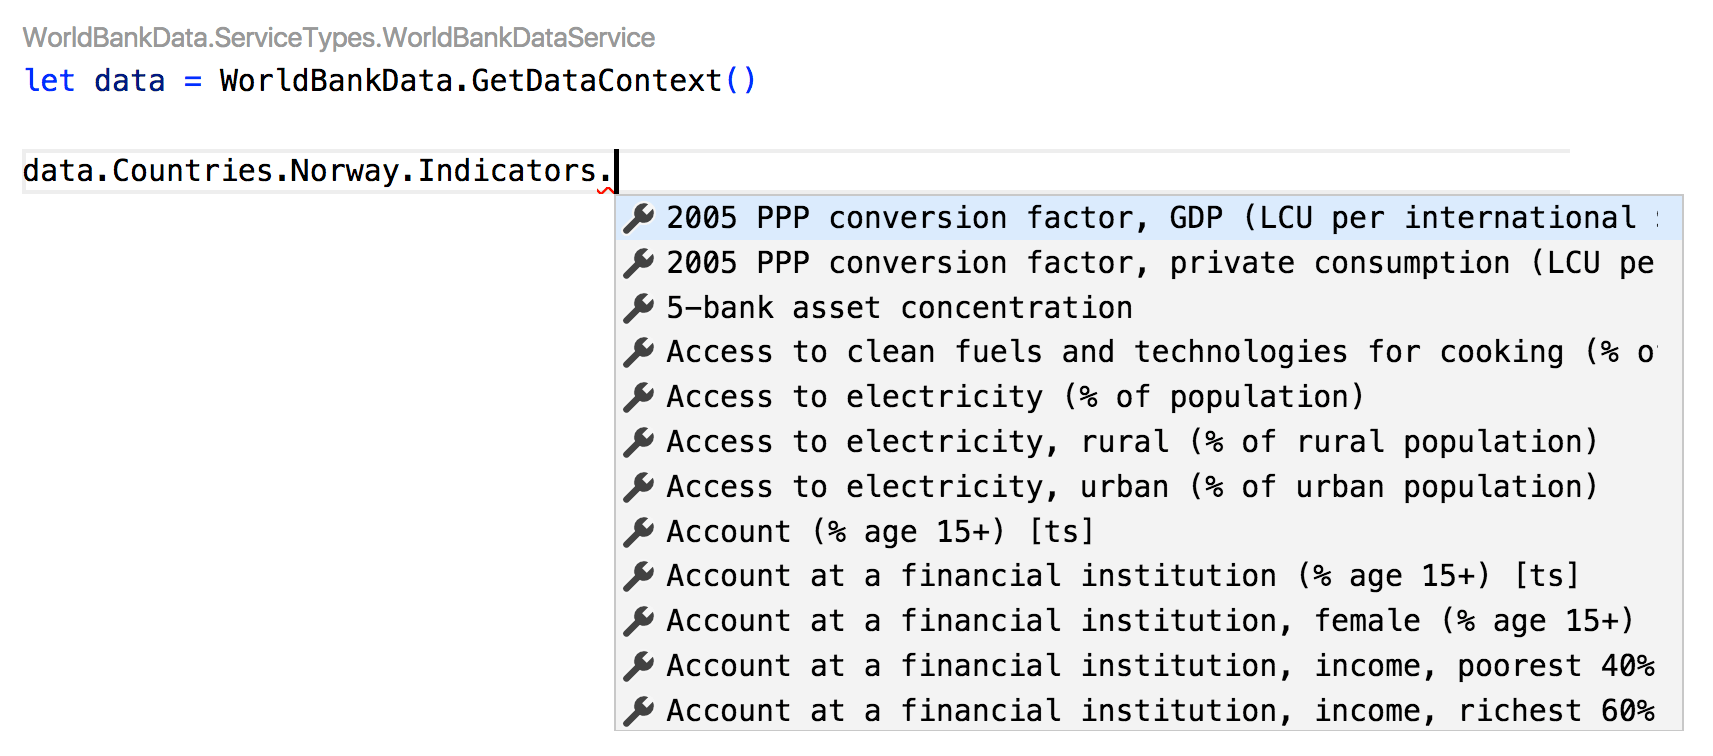
\includegraphics[width=0.8\textwidth]{worldbank_autocomplete}
\end{center}
\hspace*{-1.5in} % To get rid of some weird bottom margin
\caption{Autocomplete from the WorldBank type provider}
\label{fig:worldbank-autocomplete}
\end{figure}

A good example of a type provider which makes use of this functionality is the WorldBank type provider in \fsharpdata. As the name suggests, it provides access to the World Bank data catalog via its web API. Figure~\ref{fig:worldbank-autocomplete} shows a screenshot of the kind of autocomplete that is available when using the type provider. Having such functionality makes it quick and easy to dive into the data, and it would be very hard, or impossible, to replicate without some sort of strategy for only generating what is necessary.

While thunks as parts of generated types is clearly a very powerful feature, many of F\#s type providers are not reliant on it. If it is feasible to have all the necessary data available at once, and the generated type is not too large, delayed production of the code is not required. For example the ‹JsonProvider› from \fsharpdata\ which creates a single type hierarchy from a limited set of samples, does not need thunks. In other words, something like ‹JsonProvider› \emph{should} be possible in Rust. In chapter~\ref{chap:project-presentation} I will show how I have attempted to achieve this, but let us first look at the advantages and disadvantages of the type providers it is inspired by.

\subsection{Advantages of F\#s type providers}

% "Type checking" external resources
The most significant benefit of type providers is that they enable type-safe access to external resources, significantly improving type checking for sections of code using data from a type provider.

% Explorative programming / Tooling help
As mentioned, such type-safe access can also be achieved by manually writing the custom types, but the ease of use of a type provider makes it very easy to add a new external resource and start experimenting. Not only is the barrier of having to write boilerplate code reduced or removed, but type information gleaned through e.g. autocomplete facilitates exploration of the resource.

When working with external data, the code we write encode our assumptions about the data we are working with. E.g. if I have parsed some data into a variable ‹p› and I write code like ‹let real_name: String = p.name›, the code encodes my assumptions that the data has a field with the name ‹name›, and that said field is a string. When the types are in sync with the external data the type checking will thus check that our assumptions match the actual structure of the data. Additionally, the type checking will \emph{only} check the assumptions we state through our use of the data, which are likely to be the ones we care about.

% Detect API changes
Since these assumptions are re-checked when we re-compile this can help us not just when our assumptions change, but also when the things we are making assumptions about change. In this way a type provider like ‹JsonProvider› can help alert us about changes to remote resources while we are developing or in a continuous  integration setting.

% Encoding of otherwise impractical/impossible types
The most advanced type providers can thanks to the delayed evaluation of AST encode information that would otherwise be entirely impractical to otherwise encode in the type system. We will be hard pressed to recreate this in Rust since we will not have access to delayed evaluation, but there may be other ways that we may be able to make different trade-offs and thus explore new possibilities.

\subsection{Disadvantages of F\#s type providers}
\label{sec:disadvantages-of-type-providers}

While F\#s type providers have significant advantages, they also have some disadvantages. Type providers are essentially a code generation tool. However, type providers do not give the user access to the generated code. For type providers that use thunks, it is of course not a real option to generate the full code to be able to show it, as the \say{full} code could in fact be infinite. And if you just show the code that is already forced by the program usage, no new information is provided.

% Understanding code you cannot see

Since the difference between type providers that use delayed evaluation and those that don't is completely abstracted away from the users of the type providers, this means that there is no option to look at the generated code to understand what is going on and to inspect the structure of the parsed data. While some of the same understanding can be achieved by looking at the autocomplete suggestions it is often easier to understand the structure by looking at the actual types.

% Migration path

No access to the generated code also causes a certain amount of lock-in. Without access to the code, trying to migrate a project using type providers to manually written types forces a complete rewrite of the types provided by the type provider. In the case of parsing JSON and generating types from it there are many trade-offs that have to be made, and thus there might be reasons for such a migration as a project develops. I will come back to these trade-offs in section~\ref{sec:design-considerations}.

% Network access
A completely different issue with certain type providers is that they provide the greatest benefit with concern to the type checking when verifying the use of an external resource. However, if access to this external resource requires network access, this causes the compilation of the program to require network access for every build. Sometimes requiring network access to build is not a big concern, but other times it can be a big annoyance or even be completely out of the question.

% Build can break without code changes
Another concern many people have with type providers is that since the type checking checks if the code matches the data, the build can break if the structure of the data changes. In other words, the advantage of having our assumptions checked by the type checking also means that the build can break without any changes to the things we manage with version control. Such breakage runs contrary to the concept of reproducible builds which is a very common goal for build systems. One may counter that an external data source like an API is part of the system when it is used in a program, and as such a build failure is the correct behavior, but it is nevertheless a contentious issue.

While these very real concerns are not something that dissuade us from pursuing the significant benefits that type providers can give us, we should at the same time keep them in mind as we go forward.

%!TEX root = ../main.tex

\chapter{Presentation of the project}

Type providers have significant benefits that are worth exploring in other programming languages. I have created a project that aims to approximate the benefits of type providers in Rust.

The project is divided into five crates, as well as a crate demonstrating the use of the main crate. Most important of these are one library -- a procedural macro -- and two binaries -- a command line interface and a web interface. Figure~\ref{fig:crates} shows how the crates depend on each other.

\begin{figure}[ht!]
\vspace{2mm}
\centering
\begin{tikzpicture}[>=stealth, thick, shorten >=1pt]
\graph [layered layout, grow=up, level distance=1.3cm, nodes={draw, rectangle, rounded corners}] {
"json\_typegen\_demo" -> "json\_typegen";
"json\_typegen" -> "json\_typegen\_derive";
"json\_typegen\_derive" ->[shorten >=6pt] "json\_typegen\_shared";
"json\_typegen\_cli" -> "json\_typegen\_shared";
"json\_typegen\_web" ->[shorten >=6pt] "json\_typegen\_shared";
};
\end{tikzpicture}
\vspace{2mm}
\caption{Internal dependencies in the project}
\label{fig:crates}
\end{figure}

\section{The procedural macro}

The crate «json_typegen» provides a procedural macro of the same name, ‹json_typegen›. This macro provides an interface very similar to the type providers from \fsharpdata.

\begin{listing}[ht!]
\begin{minted}{rust}
#[macro_use]
extern crate json_typegen;
extern crate serde_json;

json_typegen!("Point", r#"{ "x": 1, "y": 2 }"#);

fn main() {
    let mut p: Point =
        serde_json::from_str(r#"{ "x": 3, "y": 5 }"#).unwrap();
    println!("deserialized = {:?}", p);
    p.x = 4;
    let serialized = serde_json::to_string(&p).unwrap();
    println!("serialized = {}", serialized);
}
\end{minted}
\caption{Usage of the procedural macro}
\label{lst:proc-macro-example}
\end{listing}

In listing~\ref{lst:proc-macro-example} a minimal example of usage of the procedural macro ‹json_typegen› is shown. This example is provided in the project source as a demo crate, «json_typegen_demo». It is worth noting that the calls to ‹unwrap› unwraps result values assuming success, and will crash the program in the event of a serialization or deserialization failure. In a real world use case we would replace these calls with error handling code.

As can be seen in the example, the procedural macro defines a type -- ‹Point› -- which is then available to be used by the programmer as any other type. The type gives type safe access to its fields, in the example ‹p.x›. Attempts to access an invalid field -- e.g. ‹p.z› -- would be a type error and thus be caught at compile time.

The procedural macro supports inline samples as shown, samples stored as local files and URLs that point to remote samples.

\begin{listing}[ht!]
\textbf{Invocation of procedural macro:}
\begin{minted}{rust}
json_typegen!("Point", r#"{ "x": 1, "y": 2 }"#);
\end{minted}
\vspace{5mm}

\textbf{Generated code:}
\begin{minted}{rust}
#[derive(Default, Debug, Clone, PartialEq,
         Serialize, Deserialize)]
struct Point {
    x: i64,
    y: i64,
}
\end{minted}
\caption{The code generated by a macro invocation}
\label{lst:basic-macro-output}
\end{listing}

Based on the JSON samples, types are inferred and Rust code with type declarations is generated. Listing~\ref{lst:basic-macro-output} shows the code generated by the macro shown in the example in listing~\ref{lst:proc-macro-example}. The types generated by «json_typegen» are all built up from the same base Rust types:

\begin{itemize}
  \item ‹Vec<T>›, growable arrays, and ‹Option<T>›, optional values, with the type parameter ‹T› always being either another of our base types or an earlier generated type.
  \item ‹i64›, 64-bit integers, and ‹f64›, 64-bit floating point numbers
  \item ‹String›, heap-allocated strings
  \item ‹bool›, boolean values
  \item ‹serde_json::Value›, «serde_json»s catchall type, as a fallback when the inference gets either not enough or conflicting information
\end{itemize}

In chapter~\ref{sec:code-generation} we will look in more detail at how these types are inferred and how the types are generated.

\subsection{Limitations compared to an actual type provider}
\label{sec:macro-limitations}

While the procedural macro looks like and in many ways works like a type provider, it is not a real type provider. For some features actual support for type providers in the compiler and the tooling would be necessary.

At the moment there is no tooling solution for Rust that provides autocomplete for types generated by procedural macros. There is reason to believe that this may change in the future. However, if this will happen at all, if it would work for the ‹json_typegen› macro specifically and when it would hypothetically be done is all mostly guesswork at this point.

Since this solution is only a procedural macro that is run at compile time and does not have knowledge of the rest of the program there is no way to implement code generation on demand that depends on how the type is used. A version of this feature would be possible to do with a procedural macro system, but would require making significant changes to the Rust compiler. It is also very possible that it is not desirable to change the macro system in this manner.

\subsubsection{Procedural macro hack}

Another limitation of the current implementation is that the macro can only be used once per scope. This is a consequence of the fact that, at the time of writing, function-like procedural macros are currently not enabled on the stable version of the Rust compiler.

To work around this limitation ‹json_typegen› is actually a normal pattern based macro. The invocation of this macro expands to the declaration of a dummy type that uses a custom derive that is implemented in «json_typegen_derive»\footnote{This hack is demonstrated in isolation, and described in more detail at \url{https://github.com/dtolnay/proc-macro-hack}}. Due to a limitation in current pattern based macros the macro is unable to create new names for each dummy type. Because of this two invocations of the macro would create two (unused) types with the same name.

\begin{listing}[ht!]
\begin{minted}{rust}
mod point {
    json_typegen!("pub Point", "point_sample.json");
}

mod vector {
    json_typegen!("pub Vector", "vector_sample.json");
}

use point::*;
use vector::*;
\end{minted}
\caption{Workaround for the single use limitation imposed by the procedural macro hack}
\label{lst:hack-workaround}
\end{listing}

In my testing thus far I have not had a use case where I needed to work around this limitation. But if necessary the easiest way is to wrap the macro invocation in module scopes, and if desired import the created types. Another workaround is to use «json_typegen_derive» directly. However in the near future\footnote{Tracking issue for procedural macros: \url{https://github.com/rust-lang/rust/issues/38356}} no hack should be needed at all as function-like procedural macros become available on the stable compiler.

\section{The command line interface}

\begin{listing}[ht!]
\textbf{Invocation of procedural macro:}
\begin{minted}{rust}
json_typegen!("Point", r#"{ "x": 1, "y": 2 }"#);
\end{minted}
\vspace{5mm}

\textbf{Equivalent run of the CLI:}
\begin{minted}{shell}
json_typegen -n Point '{ "x": 1, "y": 2 }'
\end{minted}
\caption{Equivalent uses of CLI and macro}
\label{lst:cli-and-macro}
\end{listing}

The crate «json_typegen_cli» provides a binary, ‹json_typegen›, which is a command line interface (CLI) to the same code generation as is used in the procedural macro. In other words would running the binary ‹json_typegen› and invoking the macro ‹json_typegen› output the same code if given the same input sample and options.

% Diffing of earlier code with new

\section{The web interface}

\begin{figure}[ht!]
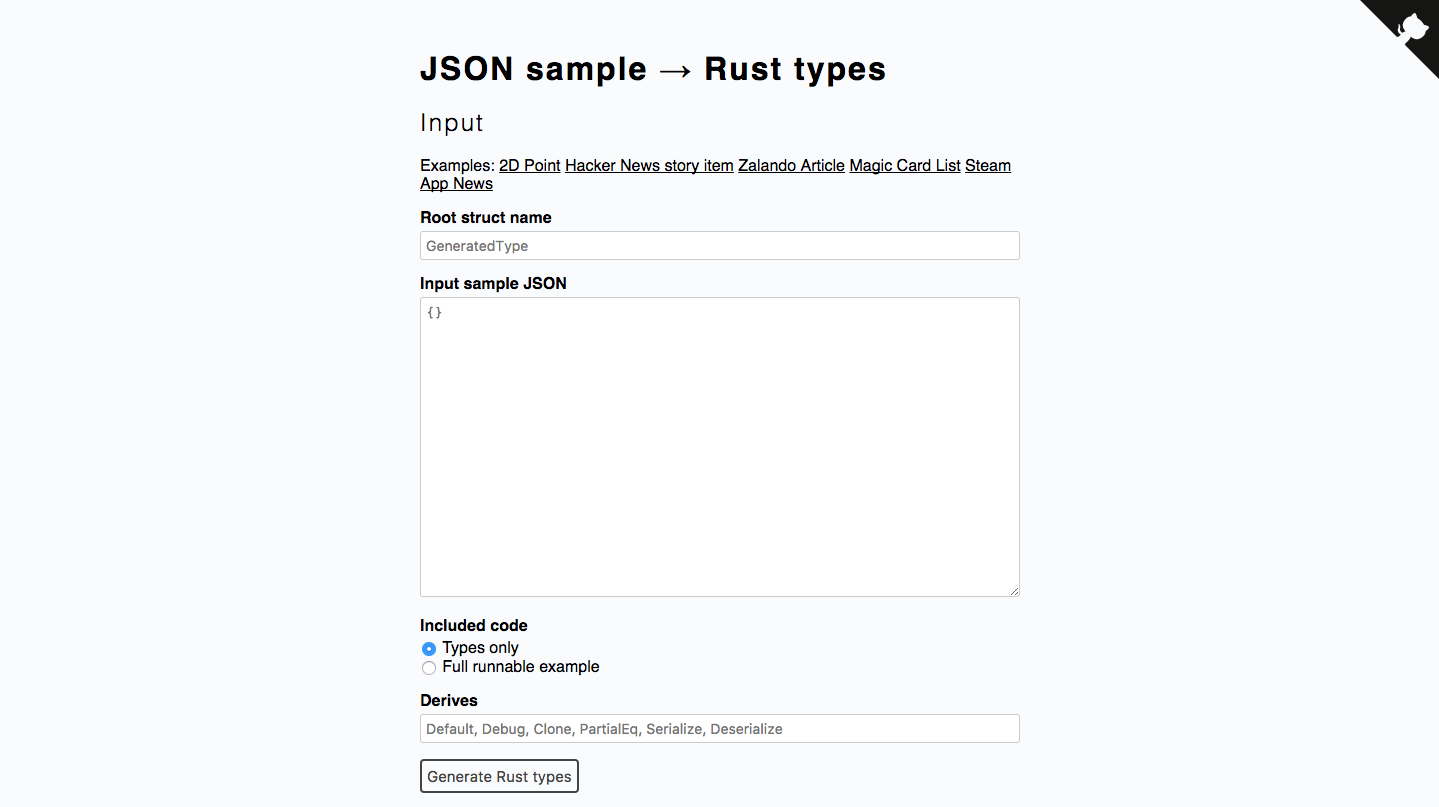
\includegraphics[width=\textwidth]{json_typegen_web}
\hspace*{-1.5in} % To get rid of some weird bottom margin
\caption{Screenshot of the web interface}
\label{fig:web-screenshot}
\end{figure}

The procedural macro and the command line interface both require the user to download and compile a somewhat significant amount of code. In small projects where the sample can be assumed not to change, this initial cost may for a lot of users seem to outweigh the benefits of the code generation.

Both of these kinds of interfaces also have a somewhat suboptimal user experience if the user wants to use a large number of configuration options. To counteract both of these problems I have made a web interface as a third way to use access the code generation logic.

The crate «json_typegen_web» provides a binary that both provides a web API for the code generation, as well as hosting the static HTML/JavaScript files providing a frontend to this API.

\section{Shared code}
\label{sec:shared-code}

As seen in figure~\ref{fig:crates} the macro, web interface and CLI all depend on a common crate, «json_typegen_shared». This crate contains the actual inference and code generation logic. The following general data flow is common to all three interfaces:

\begin{enumerate}
  \item Get the actual JSON text for the sample.
  \item Parse the JSON text into JSON values
  \item Infer type shapes from the JSON values
  \item Generate Rust code from the type shapes
\end{enumerate}

In the CLI and the web interface there is additionally a phase of formatting the generated code before the code is output to the user.

% FIXME: The rest of this section is basically just all wrong.
As mentioned in section~\ref{sec:macros} procedural macros are $ ‹TokenStream› \rightarrow ‹TokenStream› $ functions. However a ‹TokenStream› can both be parsed from a string, and written into a string. In other words we have access to both a $ ‹String› \rightarrow ‹TokenStream› $ and a $ ‹TokenStream› \rightarrow ‹String› $ function.

The different interfaces we want to provide place some requirements on what signatures we need to be able to use our code with. As mentioned, procedural macros need to have the signature $ ‹TokenStream› \rightarrow ‹TokenStream› $. A web API on the other hand must at least externally have an interface that boils down to $ ‹String› \rightarrow ‹String› $. That leaves us with two alternatives, (using $\rightarrow$ for a conversion and $\Rightarrow$ for the transformation):

\begin{align*}
‹String› \rightarrow ‹TokenStream› &\Rightarrow ‹TokenStream› \rightarrow ‹String› & \text{web} \\
                   ‹TokenStream› &\Rightarrow ‹TokenStream›                    & \text{macro} \\
\\
                        ‹String› &\Rightarrow ‹String›                         & \text{web} \\
‹TokenStream› \rightarrow ‹String› &\Rightarrow ‹String› \rightarrow ‹TokenStream› & \text{macro}
\end{align*}

In the real project things are a bit more complicated, as more types are involved, but the central point that we can consolidate different interfaces to a shared core that does the actual transformation thanks to conversion methods still stands.

\section{Synergy}
% Demonstrate how CLI or web interface can be used together with proc-macro. Explain how this then gives autocomplete etc.

Having these different interfaces provides us with some benefits that would be very difficult or impossible to achieve with only a single one.

With the three interfaces, there is a clear migration path for most use cases. A user can start with the web interface to test the code generation and see if the results fit their use case. Since it is just a normal website they can do this without having to install anything or add any dependencies.

If the code generation is suitable to their use case, copying and pasting from a website can get tedious. That combined with the additional benefits of the procedural macro will likely lead people to try the procedural macro.

As mentioned in section~\ref{sec:macro-limitations}, the procedural macro has some limitations, and as mentioned in section~\ref{sec:disadvantages-of-type-providers} even real type providers have their disadvantages. With a combination of the interfaces in this project, interesting solutions or workarounds for several of these issues are possible.

% FIXME: Unreadable sentence
Perhaps the most obvious concern that is no longer an issue is the fact that it is not possible to see expanded code with the type providers from \fsharpdata\ and the procedural macro in «json_typegen».
The two additional interfaces in this project both make it easy to see the generated code.\footnote{On nightly versions of Rust it is in fact also possible to see the resulting code after macro expansion. However, since it is fully expanded it is primarily useful for debugging purposes.}
% (also mention cargo-expand here)

The two additional interfaces also makes lock-in almost a non-issue. If a user wants to stop using «json_typegen» entirely, they can just do a final one time generation of the code. They can do this using either the web or command line interface, and replace the macro invocation with the generated code.

% autocomplete by generated code
One reason why someone might not want to use the procedural macro at the moment is the current lack of autocomplete. However, switching from the procedural macro to manually generated code means abandoning the verification against the external resource that the procedural macro gives.

\subsection{Conditional compilation}

% TODO: In Rust you can do conditional compilation by...
% #[cfg(feature = "online-samples")]
% Conditional compilation means that...

% autocomplete by generated code, but keeping benefits
To make the generated source available to editors while still keeping the benefits of the procedural macro it is possible to use conditional compilation. Listing~\ref{lst:conditional-compilation} shows an example setup where pre-generated code is used in the default build, but the pre-generated code is ignored and the procedural macro used instead when a compilation flag is enabled.

\begin{listing}[ht!]
\textbf{In the source code:}
\begin{minted}{rust}
#[cfg(not(feature = "online-samples"))]
#[derive(Default, Debug, Clone, Serialize, Deserialize)]
struct Point {
    x: i64,
    y: i64,
}

#[cfg(feature = "online-samples")]
json_typegen!("Point", "http://example.com/point.json");
\end{minted}
\vspace{5mm}

\textbf{Normal build:}
\begin{minted}{bash}
$ cargo build
\end{minted}
\vspace{5mm}

\textbf{Type checking against online samples:}
\begin{minted}{bash}
$ cargo check --features "online-samples"
\end{minted}
\caption{Conditional compilation}
\label{lst:conditional-compilation}
\end{listing}

% require network access only for verification
Using conditional compilation in this way also lets us get around the issue of requiring network access to build. If network access is the only issue we care about we don't even need to pre-generate the code, and can instead use two macro invocations -- one with a local or inline sample and one with the remote one -- as our two options.

% separate build for verification, so "normal" build still reproducible
Since the normal build in such a setup does not rely on an external resource we also get reproducible builds this way. Even if the external resource changes, it will still be possible to check out an old version of our source code and compile it. This can actually be very useful e.g. for tracking down bugs with tools like ‹git bisect›.

\section{Configurability}

There is one final problem that does not just apply to type provider like tools, but to code generation in general: Code generation always has to make some assumptions, and thus do not cover every use case and every requirement a programmer might have.

\begin{listing}[ht!]
\textbf{Sample:}
\begin{minted}{json}
{
  "registered": "2016-08-19",
  "..."
}
\end{minted}
\vspace{5mm}

\textbf{Inferred type:}
\begin{minted}{rust}
#[derive(...)]
struct Order {
    registered: String,
    ...
}
\end{minted}
\vspace{5mm}

\textbf{Desired type:}
\begin{minted}{rust}
#[derive(...)]
struct Order {
    registered: Date,
    ...
}
\end{minted}
\caption{A simple example of how generated code can fall short}
\label{lst:string-date}
\end{listing}

Listing~\ref{lst:string-date} shows a simple example of a case where the inferred type falls short of what the programmer would write by hand. There is no ‹Date› type in the Rust standard library, and as such, even with inspection of the ‹String› it would not be natural for the code generation to infer a ‹Date› type by default. While the ‹Date› type specifically may conceivably be added to the standard library in the future, the same example could apply to all manner of domain specific types.

In such cases where the generated code falls short the programmer has a few alternatives:

\begin{itemize}
  \item They can simply use the generated code as is, and convert from ‹String› to ‹Date› as necessary. If the suboptimal type is used frequently in the code though, littering the code with snippets like ‹Date::from(order.registered)› becomes frustrating pretty fast.
  \item They can customize the generated code by hand, and reapply the customizations whenever the code has to be generated again. Since this requires access to the generated code this alternative means abandoning any procedural macro or type provider. As it also makes the customized code incompatible with the generated code conditional compilation will not help here either.
  \item Finally, they can customize the generated code by hand, and completely abandon the code generation tool.
\end{itemize}

All of these alternatives have significant downsides, so if configuration of the code generation is possible, and does not come with significant downsides of its own it would in most cases be clearly preferable.

While it is clear that «json_typegen» should have at least \emph{some} configuration options, it is not obvious to what extent. It is probably not a good idea to try to cover every edge case, as such a goal could quickly lead the code to become too complex to maintain and expand. We can however make an effort to cover the most common cases, and thus increase the usefulness of the project for most people.

In the next sections I will discuss the configuration options currently available in «json_typegen» and some proposals for future expansions of these options.

\subsection{Visibility}
\label{sec:visibility}

Perhaps the simplest configuration option in «json_typegen» is type visibility. By default the generated types have no visibility specification. In Rust this means that the types are private, i.e. only accessible from the module\footnote{A file in Rust is itself a module} they are defined in, and any modules it may contain.

Private visibility for types from «json_typegen» was chosen as the default because of the inherent volatility of generating types from external resources and the fact that any change to a public type is considered a breaking API change. Thus, if the types were public by default, any change in an external sample would cause a breaking API change in users crates. If this is what the users desires, they should be free to choose so, but it is not something that should happen by accident.

To set a more public visibility for the generated types, a visibility specifier may be given along with the name for the root type. E.g. ‹json_typegen!("pub Point", ...)› would create the type ‹Point› as a public type, and if the type name ‹"pub(crate) Point"› was given, it would be created as a type visible within the current crate.

By default in «json_typegen» struct fields \say{inherit} the visibility specifier (if any) of the containing struct. This should usually be the desired behavior, but if not it can be overridden with a visibility specifier set using the option ‹field-visibility›.

\subsection{Derive list}
\label{sec:derive-list}

As explained in section~\ref{sec:traits} common behavior is specified in traits, and many of these traits can be derived -- automatically implemented -- by annotating the type with a list of traits to derive.

By default «json_typegen» annotates each generated type with the following derive list:

\begin{minted}{rust}
#[derive(Default, Debug, Clone, PartialEq, Serialize, Deserialize)]
\end{minted}

In other words will every type generated by «json_typegen» implement every trait in this list. The derive list can be overridden with the ‹derives› option. None of the traits are mandatory, but a generated type with an empty derive list would be close to useless. Since each trait has a significant effect we will look at each of the default derived traits separately. Additionally we will look at some additional traits that can be derived that a user might want to add for different use cases.

% FIXME: Show testing (appendix?)
Any unused traits and the accompanying code is eliminated by compiler optimizations when doing release builds, and so do not contribute anything to binary size. The added code generation of unused traits added very slightly to compile time in my testing, but not enough so as to be noticeable.

Since the cost for additional derived traits is so small, all the traits that are implemented for our base types\footnote{As a reminder, our base types are ‹Vec<T>›, ‹Option<T>› ‹i64›, ‹f64›, ‹String›, ‹bool› and ‹serde_json::Value›, hereafter referred to as ‹JsonVal›.} are in our default list.

\subsubsection{Serialize, Deserialize}

‹Serialize› and ‹Deserialize› are as explained in section~\ref{sec:serde} the traits that lets «serde»-compatible libraries convert to and from their various formats. It may seem like you would always want these traits, as creating types that can be serialized and deserialized is kind of \say{the point} of «json_typegen». Indeed, one would almost always want to have at least one of these traits, and sometimes both, depending on the use case. As such, in the default list both are included, but when customizing, often one can eliminate one of them. % Why?

% Converting to other formats

\subsubsection{Default, Debug, Clone}

The «Default» trait provides a no-argument constructor, creating the default value for the type. Deriving this trait creates the no-argument constructor filling in the field values with their respective default values.

This trait is in the default list mostly because it is useful for quick testing and for examples, and as such is a good aid in explorative programming. For handwritten types it usually makes more sense to manually set the default values.

Implementing the ‹Debug› trait makes the type printable via the ‹?› and \icode{\#?} debug format specifiers. E.g. an instance ‹v› of a type that implements the ‹Debug› trait is a valid argument in a statement like ‹println!("{:?}", v);›. Without implementing this trait, instances of a type can not be directly printed.

The ‹Clone› trait makes it possible to make a copy of an instance of the type by calling the ‹clone› method. For the generated types the derived implementation will result in a deep copy, which relatively speaking will be expensive. This should usually be avoided in high performance code, but is sometimes unavoidable. In quick testing and explorative programming however, it can often be quicker and easier to clone rather than try to satisfy Rusts borrow checker.

\subsubsection{Eq, PartialEq}

‹Eq› and ‹PartialEq› implements methods for comparisons that are, respectively, full and partial equivalence relations. Implementing ‹PartialEq› makes it possible to use the ‹==› and ‹!=› operators. ‹Eq› provides no additional functionality, and is just a marker trait declaring the relation to be a full equivalence relation.

‹PartialEq› is implemented for all of our base types, and is as such included in the default derive list. ‹Eq› on the other hand is not implemented for ‹f64›, floating point numbers, and ‹JsonVal›, as they themselves can contain floating point numbers.

‹f64› does not implement ‹Eq› because one of the requirements of a full equivalence relation is that it is reflexive, i.e. that every value is equal to itself. The possibility of ‹NaN› values makes ‹f64› not satisfy this property, as ‹NaN != NaN›.

While ‹f64› should not be ‹Eq›, JSON numbers are actually not allowed to be NaN or Infinity according to RFC 7159\cite[7]{RFC7159}. This means that if we could guarantee that only values from JSON data is stored in any fields that are inferred as ‹f64› we could safely make them ‹Eq›. Unfortunately, this is not something we can guarantee in Rust as immutability is a property of variable bindings, and not on fields.

‹JsonVal› actually enforces that its numbers don't contain ‹Infinite› or ‹NaN› and thus \emph{could} be ‹Eq›.

Users that know they won't have any floats or inference issues that leads to ‹JsonVal› values can add ‹Eq› to the derive list. If they have floats or ‹JsonVal› values, but are sure that any floats will come from JSON, an ‹Eq› implementation can be manually added with a ‹impl Eq for TheType {}› for each generated type. If this is something many people would do, generating these lines is something that could somewhat easily be added to «json_typegen».

\subsubsection{Hash}

Like with ‹Eq›, ‹Hash› is implemented for all of our base types except ‹f64› and ‹JsonVal›. The problem here again is ‹NaN›, but it is not as clear cut as with ‹Eq›. There are several reasonable, but no perfect solution to how floats should be hashable, so the Rust standard library provides no ‹Hash› implementation for ‹f64›. Unfortunately this leaves us with users only being able to add ‹Hash› to the derive list when they have no floats or ‹JsonVal› values (or implementing ‹Hash› manually).

This lack of ‹Hash› and ‹Eq› means that types generated with the default configuration can not be entered into any ‹HashSet› and can not be used in keys in a ‹HashMap›.

\subsubsection{Ord, PartialOrd}

% TODO: PartialOrd missing for ‹serde_json::Value›

\subsubsection{New}

In addition to the derives provided the standard library and «serde»  (which we already assume as a peer dependency) there are other custom derive libraries that can be used to add functionality to the generated types from «json_typegen». One simple such example is the «derive-new» crate, which derives a ‹new› constructor for the type with all fields as arguments. To add this functionality to all the generated types, all a user of «json_typegen» has to do is to add «derive-new» as a dependency, and add ‹New› to the derive list.

\subsubsection{Frunk: Generic, LabelledGeneric}

I won't go into detail on all the different functionality that can be added by custom derives, but one library that is of particular interest to us is «frunk». «frunk» is a library for doing functional generic programming in Rust. Among the things that it provides are two traits and accompanying derives: ‹Generic› and ‹LabelledGeneric›.

% FIXME: Add nominal/structural typing to the introduction

As explained in section~\ref{sec:rust-intro} Rust is nominally typed. This means that if we create types that have the same shape, but different names, they can not be used in place of each other, and converting between them is not all that easy. While we will look at other ways around this issue as well, ‹Generic› and ‹LabelledGeneric› provide a way to get a semblance of structural typing in Rust.

Types that implement ‹Generic› can be converted between each other if they are structurally the same, i.e. if the types have the same number of fields, with the same types, in the same order. ‹LabelledGeneric› will additionally require the fields to have the same names to allow the conversion.

\subsection{JSON pointers}
\label{sec:json-pointers}

While some configuration options like type visibility and the derive list make sense to specify globally, for the whole JSON document at once, a lot of what would be beneficial to configure has to be done on a much more granular level.

The initial case in listing~\ref{lst:string-date}, where we would want the type of a specific field to be ‹Date› rather than the inferred ‹String› is an example of where we would need such granularity.

In the example we would want to target \say{the field ‹registered› of the root object}. In our original JSON example of section~\ref{sec:json} we extracted \say{the field ‹areaCode› of the first element of the ‹phoneNumbers› field of the root object}. One of the ways we did this was with the ‹pointer› method from «serde_json» which takes as an argument something called a JSON pointer.

The JSON Pointer specification\cite{RFC6901} was originally developed along with the specification for JSON Patch\cite{RFC6902} for the HTTP PATCH method, which needed a way to specify specific elements of a JSON document. A JSON pointer is simply a string consisting of \say{reference tokens} each prefixed with a forward slash (to separate the tokens). A reference token is interpreted as either a field name or an array index, depending on whether an object or an array is encountered. So to specify \say{the field ‹registered› of the root object} we would write the JSON pointer ‹"/registered"›. And the JSON pointer we used in section~\ref{sec:json} to extract \say{the field ‹areaCode› of the first element of the ‹phoneNumbers› field of the root object} was ‹"/phoneNumbers/0/areaCode"›.

Since JSON pointers are representable as simple strings they are easy to use as arguments to both macros or in command line invocations. Since they are already used by «serde_json» it also makes sense to use JSON pointers rather than introduce yet another way to reference data originating from JSON.

Since JSON pointers are a \say{stringly typed} way to talk about data, it may seem strange to use them in a project that is so focused on type safety. There is however a significant distinction in using such code at compile time and at runtime. The criticism of \say{stringly typed} code in a strongly typed language is that it ends up reverting to a state where errors are discovered at runtime. If configuration for «json_typegen» specified through a JSON pointer does not apply to any of the sample, this can be known well before runtime, when generating the code (i.e. at compile time for the macro), and a warning or an error can be shown to the user at that point in time.

\placeholder{Actually show some examples of using JSON pointers for configuration}

Due to the use case the JSON pointer specification was developed for, there is however a rather glaring omission when it comes to adapting it to our use case. The complete lack of any wildcard.

% TODO: Existing solutions to lack of wildcard

\subsection{Cost of configurability}

While extensive configurability has significant benefits, there are also significant costs. Every configuration option a project adds increases its exposed API surface. The more exposed API surface we have, the more difficult maintenance and continued development becomes with making breaking changes.

With multiple interfaces each added configuration option in the shared code also needs to be exposed and handled multiple times. E.g. for just the web interface, each option needs to be added to the HTML form, added to the communication with the backend and be handled by the backend. Then similar work has to be done for the command line interface and the procedural macro.

% Problems with adding a lot of configuration in a project with multiple interfaces

% TODO: Approaches to working around this by generating parts of the interfaces based on the Config data type.

\section{Improving the synergy}
\label{sec:improving-synergy}

While the synergy between the different interfaces is already quite good there are ways in which it could be improved.

Since many of the use cases involve moving between the interfaces, making the transition between them as smooth as possible is an important part of the total user experience of the project.

While the "native" user experiences of the interfaces are quite different, with different strengths and weaknesses, the central functionality they provide, including configurability, should be the same. However if a user have taken extensive advantage of this configurability, having to replicate the same configuration settings from one interface in another can erase the convenience the other interface would provide.

For example is one of the use cases for the web interface to easily be able to see the generated code when using the procedural macro. However, a option in the macro is expressed as code, while the natural interface for the website is a form. For this specific use case it would be much nicer to just be able to copy the macro invocation as text, and get the output without having to use the form. In other words would it be convenient if the web interface would be able to read the macro syntax as an additional input format. Use cases for the CLI would benefit much the same way if a macro invocation could be used directly to generate code. What I propose is essentially to use the macro syntax as an ad hoc configuration interchange format.

If the web interface additionally can output in the macro syntax we get easy transitions that cover what I think are the most likely user stories:

\begin{itemize}
  \item Just discovered the project, and having tested in web interface, want to start using the macro: web $\rightarrow$ macro.
  \item Using the macro, but want to see the generated code for quick debugging: macro $\rightarrow$ web.
  \item Using the macro, but want to use CLI for autocomplete or other reasons for conditional compilation: macro $\rightarrow$ CLI.
\end{itemize}

\begin{figure}[ht!]
\vspace{2mm}
\centering
\begin{tikzpicture}[>=stealth, thick, shorten >=1pt, node distance=3.5cm, auto, scale=3]
  \tikzstyle{every state}=[draw, minimum size=1.5cm]

  \node[state] (cli)   at (0,0)       {CLI};
  \node[state] (macro) at (1,0)       {macro};
  \node[state] (web)   at (0.5,0.866) {web};

  \path[->] (web) edge [bend right=20] (cli);
  \path[->] (web) edge [bend right=20] (macro);
  \path[->] (macro) edge [bend right=20] (cli);
  \path[->] (macro) edge [bend right=20] (web);
  \path[->, dashed] (cli) edge [bend right=20] (web);
  \path[->, dashed] (cli) edge [bend right=20] (macro);
\end{tikzpicture}
\vspace{2mm}
\caption{Transitions enabled by CLI and web interface being able to read, and web interface being able to write, macro syntax. The dashed lines show transitions that require the use of the macro syntax as the configuration format, and not just as the interchange format.}
\label{fig:transitions}
\end{figure}

The way I've described how the procedural macros work in section~\ref{sec:shared-code} it may seem like we could get at least parsing of the macro \say{for free}. Unfortunately this is currently not the case. Since the current macro is not a procedural macro, we do not ever use the macro code itself as input, but rather what it expands to. However, any parsing code written for configuration interchange may very well be directly usable once normal procedural macros are available on the stable compiler and it is time to transition the «json_typegen» macro.

% Easy way to transition between interfaces. E.g. copy-paste macro into web interface to see result. Output macro in web interface that is equivalent to the current form input. Etc.
% Doing this would mean essentially writing a minimal macro parser and generator. I.e.
% MacroString -> (SampleSource, Config)
% (SampleSource, Config) -> MacroString

% TODO: Have CLI be able to set up conditional compilation. Maybe also web interface?

\placeholder{Describe idea behind \url{https://github.com/evestera/atom-json-typegen} and superficially how it works/can work.}

%!TEX root = ../main.tex

\chapter{Code generation}
\label{sec:code-generation}

\begin{picture}(0,0)
\put(150,85){\hbox{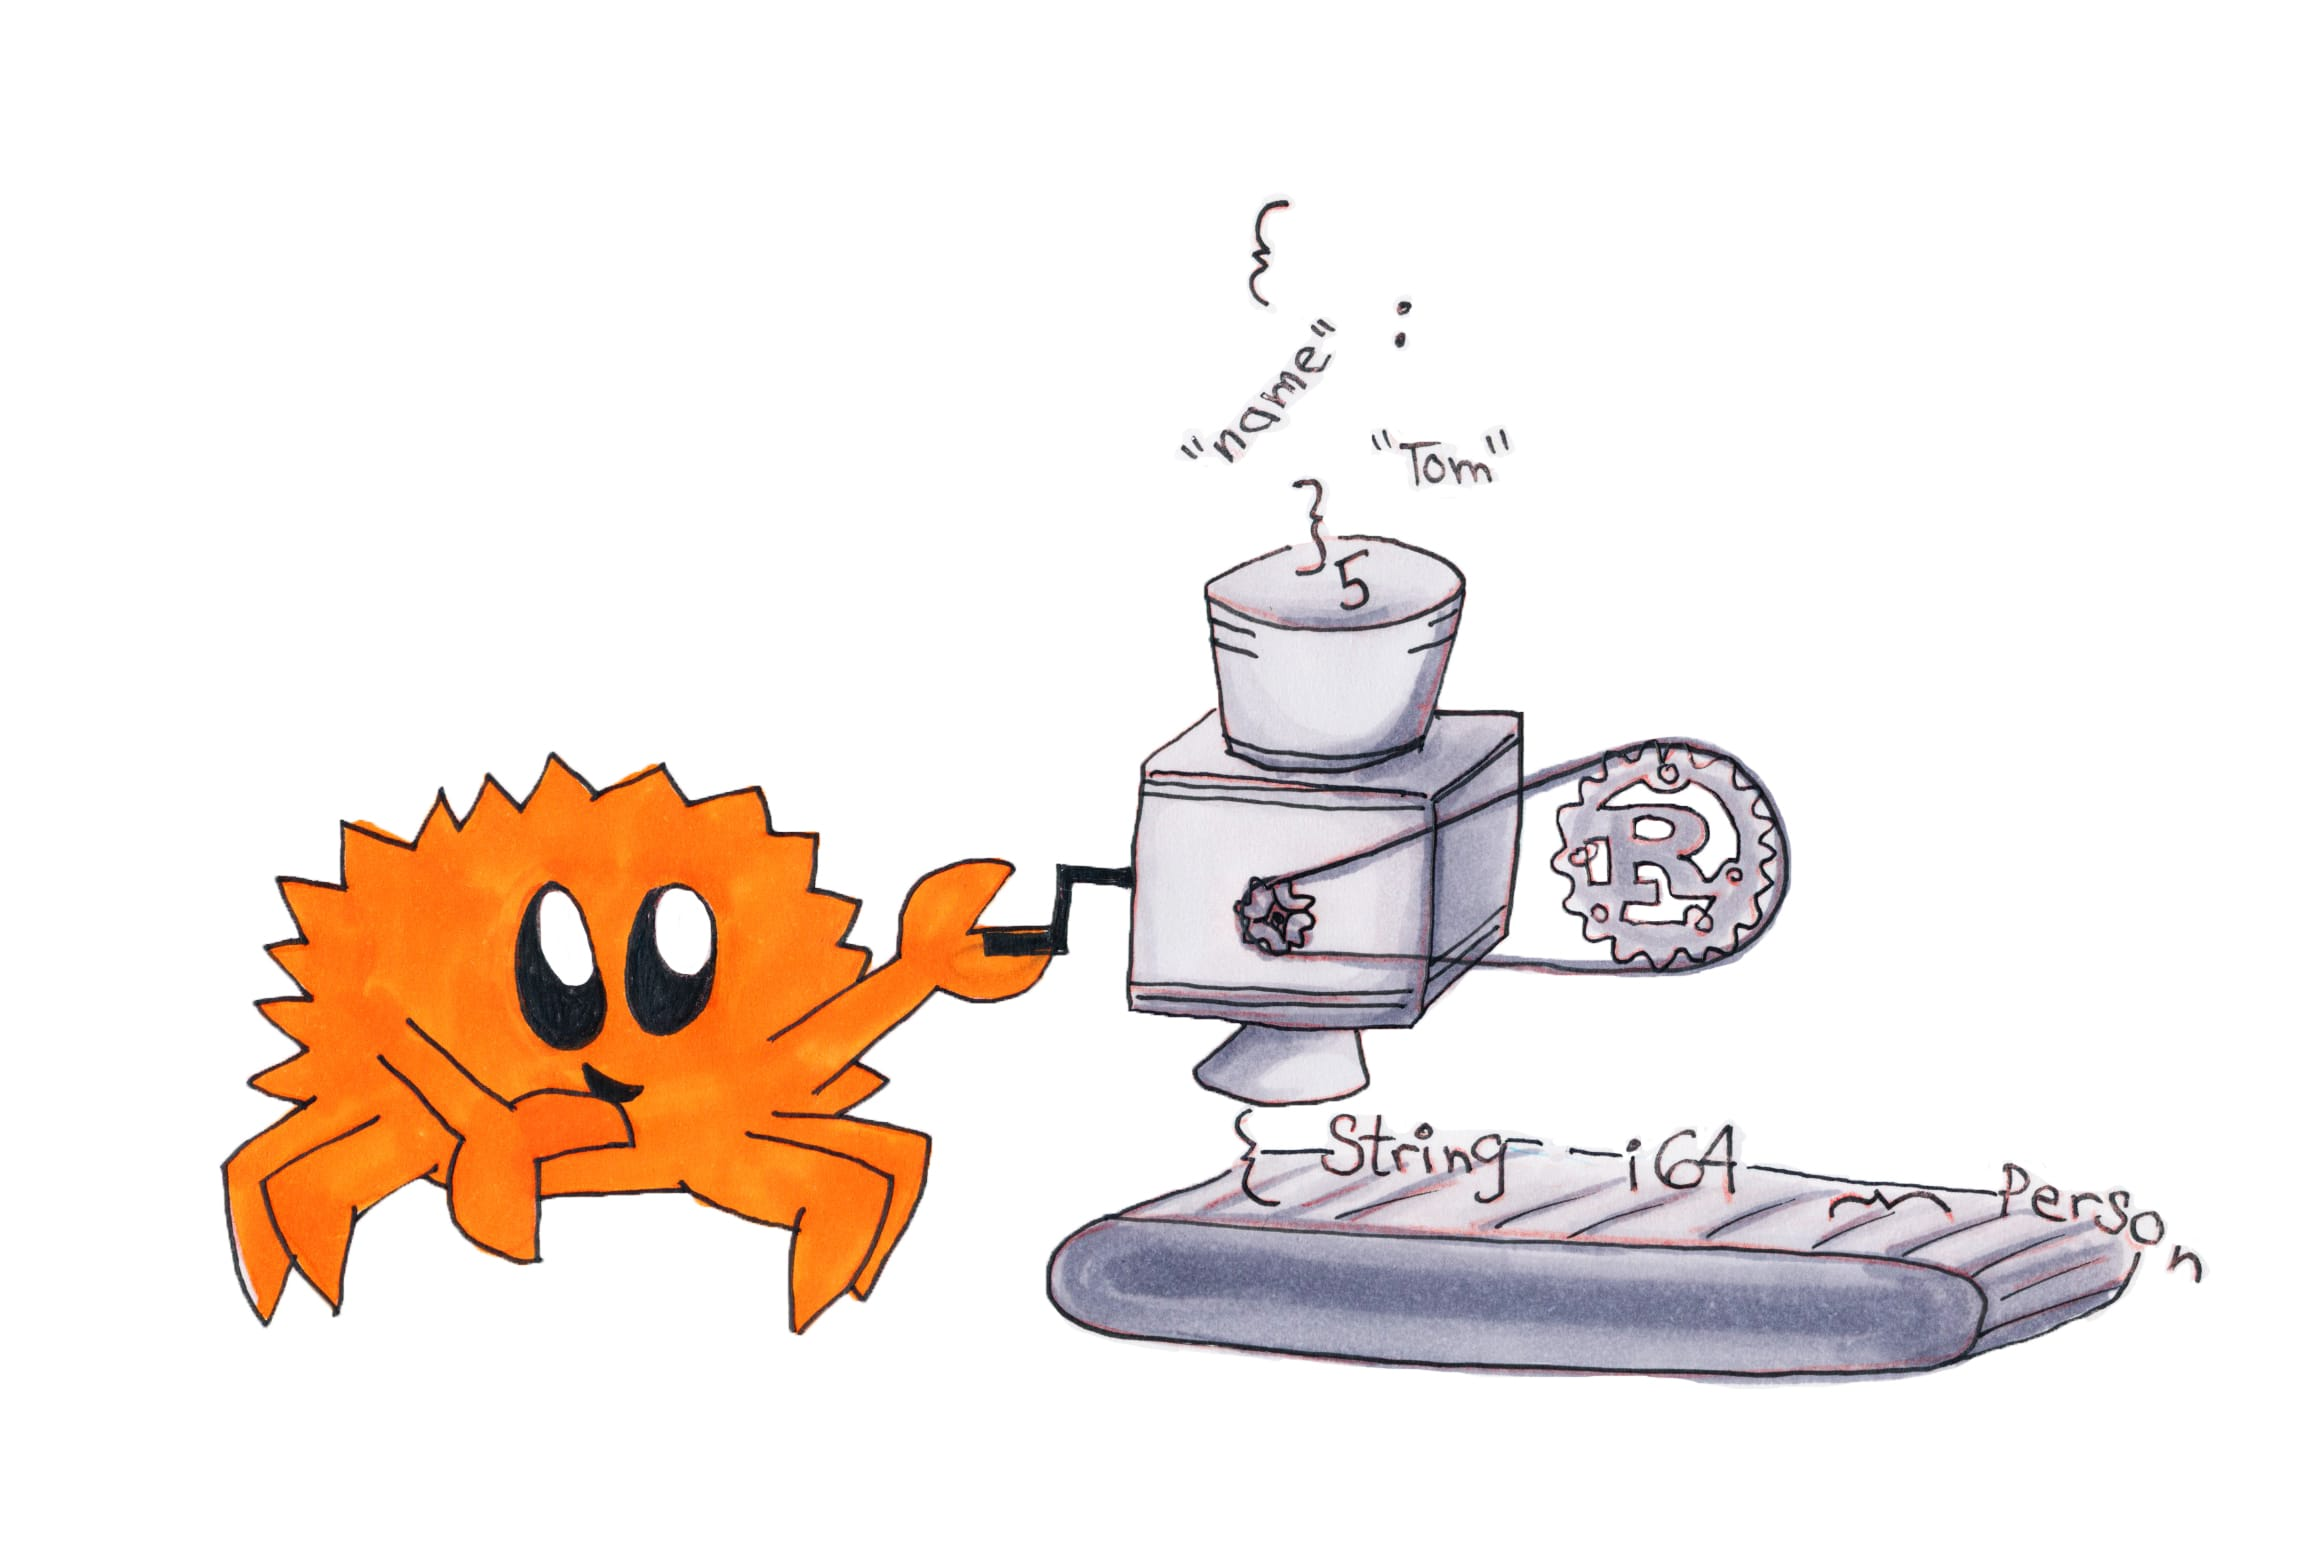
\includegraphics[width=8.5cm, angle=0, trim=40 100 40 40, clip]{ferris/machine}}}
\end{picture}
\vspace{-1cm}

Once a JSON sample has been retrieved and parsed using «serde_json» into the catchall type ‹serde_json::Value›, «json_typegen» is ready to begin inference and code generation. In this chapter we will look at the details of these three stages:

\begin{itemize}
  \item First, a generalized \say{shape} is inferred from the JSON values.
  \item Then this inference is enhanced in intermediary passes.
  \item Finally, Rust code is generated based on the inferred shapes.
\end{itemize}

To begin with I will present a basic version of the inference algorithm and code generation, before looking at how this system can be extended in various ways.

\section{Shape inference}
\label{sec:shape-inference}

The shape inference is based on the algorithms used in \fsharpdata\ as presented in the paper \emph{Types from Data: Making Structured Data First-class Citizens in F\#}\cite{fsharp-types-from-data}. As done in this paper I will use the term shape for the intermediate representation of the inference data, to avoid confusion with actual programming language types.

The goal of the shape inference is to infer generalized shapes from the samples which can then later be used for generating code. These shapes are intended to be general enough to not be tied to inference from JSON -- \fsharpdata\ also does inference for CSV and XML -- and not tied to the generation of any particular type of programming language. Rust code for the basic version of the shape inference can be seen in appendix~\ref{app:inference-code}.

\subsection{Values and shapes}

The inference thus works with two types. The JSON sample, in our case parsed into a ‹serde_json::Value› -- as was shown in Listing~\ref{lst:valueenum} -- and the shape type. An abstract version of ‹serde_json::Value›, with value variables \omega, and our shape type, with shape variables \sigma, can be written as follows:

\begin{align*}
\omega ::=  &\ ‹Null› \mid ‹Bool(›b‹)› \mid ‹Number(›n‹)› \mid ‹String(›s‹)› \\
       \mid &\ ‹Array(›[\omega_1, \cdots, \omega_n]‹)› \mid ‹Object(›\{ k_1 : \omega_1, \cdots, k_n : \omega_n \}‹)›\\
\\
\sigma ::=  &\ ‹any› \mid \bot \mid ‹bool› \mid ‹string› \mid ‹int› \mid ‹float› \\
       \mid &\ ‹optional(›\sigma‹)› \mid \vect{\sigma} \mid \recd{ k_1 : \sigma_1, \cdots, k_n : \sigma_n }
\end{align*}

To be clear about how notation is disambiguated: $[a, b, c]$ is an actual sequence of items, while $\vect{a}$ is the \emph{shape} representing a sequence/list.\footnote{In «Types from Data» the notation $\vect{a}$ is used for a different purpose in a section of the paper we will not look at here.} Likewise $\{ k_1 : v_1, \cdots, k_n : v_n \}$ is a map-like collection, while $\recd{ k_1 : \sigma_1, \cdots, k_n : \sigma_n }$ is the \emph{shape} representing a record/object/struct.

For an intuitive understanding of the more abstract shapes it is helpful to think of what kind of knowledge each shape represents. $\bot$ (read as \say{bottom}) represents the complete lack of knowledge about what type should be inferred. $‹optional(›\sigma‹)›$ represents the knowledge that a type may sometimes be ‹null› or a field may not always be there, i.e. that it is nullable or optional. So $‹optional(›\bot‹)›$ tells us that a type is optional, but that we know nothing else of about its type. The ‹any› shape, on the other hand, represents conflicting information. If we end up with the ‹any› shape it means that the information we have received is not representable by any of the other alternatives. E.g. a type that can be both a ‹string› and an ‹int›.

% Differences from algorithm as presented in Types from Data
Unlike in «Types from Data», to preserve information and let any choice be made in the code generation step, lists\footnote{\ldots\ and with extensions, other collections.} are not considered nullable. In other words, the inference can infer the shape $‹optional(›\vect{\sigma}‹)›$, but it is up to the code generation to decide how to handle the shape. In the default code generation, ‹Option<Vec<T>>› will not be generated, but this can be enabled by configuration (‹optional_collections›).

With this change, a separate ‹null› shape, which the original algorithm has, is no longer necessary. Instead, $\bot$ is not considered nullable either, and $‹optional(›\bot‹)›$ serves the purpose of ‹null›.

\subsection{From values to shapes}

\begin{figure}[ht!]
\begin{align*}
\shap(‹Null›)          &= ‹optional(›\bot‹)› \\
\shap(‹Bool(›b‹)›)     &= ‹bool› \\
\shap(‹Number(›n‹)›)   &= \begin{cases}
  ‹int›   & \text{if } n \in \mathbb{Z} \\
  ‹float› & \text{otherwise}
\end{cases}\\
\shap(‹String(›s‹)›)   &= ‹string› \\
\shap(‹Array(›[\omega_1, \cdots, \omega_n]‹)›) &= \vect{ \fold(\csh, \bot, [\shap(\omega_1), \cdots, \shap(\omega_n)]) } \\
\shap(‹Object(›\{ k_1 : \omega_1, \cdots, k_n : \omega_n \}‹)›) &= \recd{ k_1 : \shap(\omega_1), \cdots, k_n : \shap(\omega_n) }
\end{align*}
\caption{$\shap(\omega)$, the function converting JSON values to shapes}
\label{fig:shap}
\end{figure}

The main inference function $\shap(\omega)$, shown in Figure~\ref{fig:shap} takes as its input a value and produces a shape. Values containing other values are converted by applying $\shap$ recursively.

$\fold(\textit{function}, \textit{base}, \textit{sequence})$ is the fold operator\cite{fold-tutorial}, common in functional programming (and available on iterators in Rust). In this case, it reduces a sequence of shapes to a single shape by finding a common shape with the $\csh(\sigma_1, \sigma_2)$ function, which we will look at in the next section. The initial shape is $\bot$, which means that an empty ‹Array› will be represented as the shape $\vect{\bot}$.

\subsection{Finding common shapes}

\begin{figure}[ht!]
\begin{align*}
\csh(\sigma, \sigma)     &=  \sigma          & (eq) \\
\csh(\sigma, \bot)       &=  \sigma          & (bottom) \\
\csh(‹int›, ‹float›)     &= ‹float›          & (num) \\
\csh(\sigma_1, ‹optional(›\sigma_2‹)›) &= \opt(\csh(\sigma_1, \sigma_2))  & (opt) \\
\csh(\vect{\sigma_1}, \vect{\sigma_2}) &= \vect{\csh(\sigma_1, \sigma_2)} & (arr) \\
\csh(\sigma_1 = \recd{ \cdots }, \sigma_2 = \recd{ \cdots }) &= \cfs(\sigma_1, \sigma_2) & (obj) \\
\csh(\sigma_1, \sigma_2) &= ‹any›            & (any)
\end{align*}
\caption{$\csh(\sigma_1, \sigma_2)$, the common shape function}
\label{fig:csh}
\end{figure}

Sometimes multiple elements must be represented by the same shape, e.g. a single shape representing all the elements of an array. Figure~\ref{fig:csh} shows the function $\csh(\sigma_1, \sigma_2)$ which for two shapes finds a common shape which can represent them both. Order of arguments does not matter, so for every rule $\csh(a, b)$ the rule $\csh(b, a)$ is the same.

$\csh(\sigma_1, \sigma_2)$ defines a partial order for the set of shapes, where if $\csh(\sigma_1, \sigma_2) \vdash \sigma_3$, $\sigma_1 \sqsubseteq \sigma_3$ and $\sigma_2 \sqsubseteq \sigma_3$. The relation $\sqsubseteq$ can be understood as the \say{can be represented by}-relation. E.g. $ ‹float› \not\sqsubseteq ‹int› $, but $ ‹int› \sqsubseteq ‹float› $ (and also $ ‹int› \sqsubseteq ‹int› $).

\begin{figure}[ht!]
\vspace{2mm}
\centering
\begin{tikzpicture}[>=stealth, thick, shorten >=1pt, auto, scale=1.2]
  \node (bot)     at (8,0) {\bot};
  \node (bot?)    at (9,1) {\bot?};
  \node (int)     at (0,2) {‹int›};
  \node (int?)    at (1,3) {‹int›?};
  \node (float)   at (0,4) {‹float›};
  \node (float?)  at (1,5) {‹float›?};
  \node (bool)    at (2,2) {‹bool›};
  \node (bool?)   at (3,3) {‹bool›?};
  \node (string)  at (4,2) {‹string›};
  \node (string?) at (5,3) {‹string›?};
  \node (arr)     at (6,2) {$\vect{\sigma}$};
  \node (arr?)    at (7,3) {$\vect{\sigma}$?};
  \node (obj)     at (8,2) {$\recd{\cdots}$};
  \node (obj?)    at (9,3) {$\recd{\cdots}$?};
  \node (any)     at (9,6) {‹any›};

  \begin{scope}[on background layer]
    \path[->] (bot)    edge (bot?);
    \path[->] (int)    edge (int?);
    \path[->] (float)  edge (float?);
    \path[->] (bool)   edge (bool?);
    \path[->] (string) edge (string?);
    \path[->] (arr)    edge (arr?);
    \path[->] (obj)    edge (obj?);

    \path[]   (bot)    edge (0,0);
    \path[->] (0,0)    edge (int);
    \path[->] (2,0)    edge (bool);
    \path[->] (4,0)    edge (string);
    \path[->] (6,0)    edge (arr);
    \path[->] (bot)    edge (obj);
    \path[->] (int)    edge (float);

    \path[    dashed] (bot?) edge (1,1);
    \path[->, dashed] (1,1)  edge (int?);
    \path[->, dashed] (3,1)  edge (bool?);
    \path[->, dashed] (5,1)  edge (string?);
    \path[->, dashed] (7,1)  edge (arr?);
    \path[->, dashed] (bot?) edge (obj?);
    \path[->, dashed] (int?) edge (float?);

    \path[]   (float?)  edge (9,5);
    \path[]   (bool?)   edge (3,5);
    \path[]   (string?) edge (5,5);
    \path[]   (arr?)    edge (7,5);
    \path[->] (obj?)    edge (any);
  \end{scope}
\end{tikzpicture}
\vspace{2mm}
\caption{Hasse diagram for the partial order. For compactness $\sigma$? is used for $‹optional(›\sigma‹)›$. Dashed lines are only for visual clarity.}
\label{fig:poset}
\end{figure}

Figure~\ref{fig:poset} shows an incomplete Hasse diagram for the partially ordered set given by $\sqsubseteq$ on the set of shapes. The internal ordering of list and record shapes, $\vect{\sigma}$ and $\recd{\cdots}$, is not shown.

\begin{figure}[ht!]
\begin{align*}
\opt(‹any›)                &= ‹any› \\
\opt(‹optional(›\sigma‹)›) &= ‹optional(›\sigma‹)› \\
\opt(\sigma)               &= ‹optional(›\sigma‹)›
\end{align*}
\caption{$\opt(\sigma)$, the function ensuring optionality/nullability of shapes}
\label{fig:opt}
\end{figure}

When we are working with optional shapes, we want optionality to be a boolean property, i.e. either something is optional, or it is not. For any shape $\sigma$ that already encodes the possibility of values that are missing or ‹null›, $\opt(\sigma)$, as shown in Figure~\ref{fig:opt}, is simply a no-op.

\begin{figure}[ht!]
\begin{gather*}
\cfs(\sigma_1 = \recd{ k_1 : v_1, \cdots, k_n : v_n }, \sigma_2 = \recd{ k_1 : v'_1, \cdots, k_n : v'_n }) = \\
\recd[\bigg]{
\forall\ k_n \in \sigma_1 \cup \sigma_2 .\ k_n : \begin{cases}
  \csh(v_n, v'_n) & \text{if } k_n \in \sigma_1 \cap \sigma_2 \\
  \opt(v_n) & \text{if } k_n \notin \sigma_2 \\
  \opt(v'_n) & \text{if } k_n \notin \sigma_1
\end{cases}
}
\end{gather*}
\caption{$\cfs(\sigma_1, \sigma_2)$, the function for finding the common shape of two records}
\label{fig:cfs}
\end{figure}

Figure~\ref{fig:cfs} shows how the common shape of two record shapes is found by finding the common shapes of its fields. For keys that are not present in both records, the shape that is present is optional/nullable. Note that in «Types from Data», records have row variables\cite{row-types} so that all records can be considered to have the same keys. To minimize the number of new concepts needed to understand the basic algorithm I have chosen this slightly less elegant notation in Figure~\ref{fig:cfs} instead. Informally, every key present in either of the input record shapes will be present in the output record shape. For every field, if the field is found in both record shapes, the shape of the field in the output is the common shape of the shapes for the corresponding fields in the input. If the field is found in only one of the input shapes, the corresponding field in the output shape must be optional.

\section{Intermediary passes}

In the basic version of the algorithm, there are no intermediary passes. These passes are mainly a result of extensions of the algorithm. The extensions come about for two main reasons: Improving the code to more closely resemble hand-written code, and adding configurability of the inference and code generation.

We will look at these extensions and their consequences for the algorithm in section~\ref{sec:extensions}.

\section{Generating Rust types}

Once a shape tree has been inferred from the sample and intermediate passes have been run to improve the inferred shapes, the shape tree is used to generate Rust code.

The main function takes as its input some path information, used for naming any generated types, and a shape. The function pattern matches on the shape and produces as its output a tuple: The name of the type representing the shape, and potentially some code generated to declare the returned type.

Code is generated via quasiquotation, using a macro ‹quote!› from the «quote»\cite{quote} library.

% TODO: Expand this section

\subsection{Type and field names}

Up to the point of code generation, JSON field names have been preserved as they were in the original JSON. These field names are used to create both field names for the generated types, as well as type names for any nested types. However, as mentioned in section~\ref{sec:json}, the JSON field names can be completely arbitrary strings, while the field names and type names we generated must conform to Rust rules and conventions for identifiers.

The generated names are restricted to consist of \say{words} of alphanumeric ASCII characters, and the complete name must start with a letter. Type names are \say{PascalCased}, i.e. concatenated, with the first letter of each word upper-cased, and field names are \say{snake\_cased}, i.e. all lower case, with words separated by an underscore. For some fields, nothing of the original name remains after restrictions are applied, and we have to resort to fallback names like ‹GeneratedType›.

\begin{listing}[ht!]
\textbf{Sample:}
\begin{minted}{json}
{
  "one two": { " ": 5, "?": 2 }
}
\end{minted}
\vspace{5mm}

\textbf{Generated types:}
\begin{minted}{rust}
struct Root {
    #[serde(rename = "one two")]
    one_two: OneTwo,
}

struct OneTwo {
    #[serde(rename = " ")]
    field: i64,
    #[serde(rename = "?")]
    field2: i64,
}
\end{minted}
\caption{Field and type renaming}
\label{lst:names}
\end{listing}

Additionally the generated types cannot collide with Rust keywords or each other. Collisions with keywords are solved by appending a word describing its use, like ‹field›, so the field ‹"type"› becomes ‹type_field›. Collisions between generated names are solved by adding an incrementing counter to the name.

For field names, if the Rust field name does not match the JSON field name an annotation to relay this information to «Serde» is added to the field. Listing~\ref{lst:names} shows an example with several of these issues at once.

\subsection{Generation of a runnable program}

In addition to just generating the types themselves, the code generation can also generate a complete, runnable Rust program. In addition to the generated types, the runnable program contains the necessary imports and a main function showing how to use «serde_json» to deserialize and serialize into the generated types.

The generation of a full program is mainly for documentation and demonstration purposes in the web interface. Using a button in the web interface the generated code can be directly compiled and run in the online Rust playground.

\subsection{Use of derivable traits}
\label{sec:use-of-derivable-traits}

As outlined in section~\ref{sec:derive-list} a lot of the functionality of «json_typegen» is founded on the fact that many traits can be derived -- i.e. that they can be implemented by just adding their name to a list -- and that this works even for complex generated types.

The fact that this is possible relies on two important preconditions:

\begin{enumerate}
  \item That our generated types are composed of either our base types, or other generated types. I.e. that every leaf in our generated type tree is one of our base types.
  \item That every trait in our derive list is derivable and implemented for each of our base types.
\end{enumerate}

% Proof of "every leaf in our generated type tree is one of our base types" necessary?

% Proof by structural induction here of the claim that this then makes deriving safe for complex types?

Both of these preconditions can be broken by the user if the right configuration option is provided. As explained in section~\ref{sec:derive-list}, the derive list can be overridden. This can obviously break our second precondition, either if a trait is not implemented for one of our base types, or for that matter if the trait is not derivable at all. There are also ways configuration can introduce new, essentially opaque, types into the code generation. These new types essentially become new base types, and as such can easily break our first precondition.

If a user breaks our preconditions in this way and this leads to a compiler error. The messages when a derive fails are clear and should make it quite obvious to the user what the problem is. With this in mind, I think letting the user break these preconditions is an acceptable trade-off for the benefit these configurations provide.

While letting the user break these preconditions is acceptable, care has to be taken to preserve these preconditions when extending the basic system. To make the source of any errors obvious, no derive errors should be possible that does not directly mention a trait or type explicitly specified by the user. E.g. if the system is extended with sets, enabling this extension should not be possible without explicitly choosing a target type if doing so breaks the preconditions.

\subsection{Strictness of deserialization}
\label{sec:design-considerations}

While the types we generate should match the samples they are generated from, and any JSON text that matches their structure, there is always the possibility that the actual JSON we encounter at runtime does not perfectly match what we inferred.

\subsubsection{Mismatched field types}

If a field has entirely the wrong type, e.g. an object where we expect a number, deserialization has to fail with an error, as discovering such type issues as early as possible is a big part of the reason to deserialize to strong types. There are, however, some types we \emph{could} conceivably coerce between. E.g. the string value ‹"3.5"› could be parsed and coerced into a ‹f64› field. While I have some ideas for extensions for specific instances like strings to number, I have no plans for supporting coercing data at runtime in an ad-hoc fashion.

When it comes to how we handle fields that are either missing or that we never saw in inference there are some choices to be made.

\subsubsection{Missing fields}

In the inference we detect potentially missing fields and encode this information into the shapes. By default, the code generation maps $‹optional(›\sigma‹)›$ to ‹Option<T>›, and if any field that was not inferred to be optional is missing, deserialization fails. However, another way to handle missing fields that «Serde» supports is to use the default value provided by an implementation of the ‹Default› trait. I.e. if a string is missing, use the empty string, if an integer is missing use 0, and so on. By enabling this functionality for every field a user could make sure deserialization never fails due to a missing field.

\subsubsection{Additional fields}

By default, if «Serde» tries to deserialize and the data has an additional field that the target type does not have, the additional field is just ignored. This matches well with our intent with type providers, in that we only want to check the assumptions we actually make. However, it is also possible to make such additional fields cause deserialization to fail.

\section{Extensions}
\label{sec:extensions}

As have been mentioned earlier, there are several ways to extend this basic setup to better align with what handwritten code would look like. We will now look at a few such extensions. For the sake of simplicity, we will mostly not go into the details of how these extensions interact or the complete extended algorithms, focusing instead on each extension by itself.

\subsection{Tagged any types}
\label{sec:tagged-any}

In addition to the basic inference algorithm described in section~\ref{sec:shape-inference}, «Types From Data»\cite{fsharp-types-from-data} also describes an extension it calls \say{labelled top shapes} for providing a better fallback than the general ‹any› shape.

In the basic algorithm, if the least upper bound given by $\csh(\sigma_1, \sigma_2)$ is ‹any›, we throw away the information we have about why we had to use ‹any›, i.e. $\sigma_1$ and $\sigma_2$. The basic concept of this extension is to instead incorporate this information into a top type $‹anyof(›\sigma_1, {\cdots}, \sigma_n‹)›$. This can then be used in the code generation to e.g. create enumerated types with custom types inside.

% TODO: Show how a type generated from an anyof shape could look

% TODO: HTML or XML example

This extension is absolutely vital for making the algorithm work well with XML and HTML. In these formats heterogeneous collections with easily disambiguated types are abundant. For «json_typegen», the extension is still useful, but less important than some other extensions.

\subsection{JSON pointer hints and configuration}
\label{sec:ext-json-pointers}

As outlined in section~\ref{sec:json-pointers} we can use JSON pointers to specify configuration options and hints (hereafter referred to as just options) to the inference that are specific to just a part of the JSON sample.

Actually applying these options require some modifications to the basic version of the algorithm. However, the options are not all applied the same way or at the same time. Some have to be applied during inference, some are best applied as intermediate transformations between inference and code generation, and some have to be applied during the code generation. This means that while we start with a simple list of options, we have to do some pre-processing of the options before running the algorithm with them.

The pointer options must then be threaded through our inference and code generation functions, and applied as they match.

A pointer option is a 3-tuple of a pointer, an option name, and an option value. For applying the option we transform the pointer into a list of keys. E.g. the pointer ‹"/field1/field2"› is converted to the list of keys $[‹"field1"›, ‹"field2"›]$. For


% some in inference, some as intermediate steps, some for code generation

% consequences of plain pointers (and array indexes), full wildcards and partial wildcards

% same_as, ids to see which types are the same

\subsection{More number types}
\label{sec:unsigned}

By default, our code generation only uses ‹i64› for integers and ‹f64› for floating point numbers. While these are good defaults, there are several other number types that could be used. In particular, the Rust standard library provides types for unsigned numbers, e.g. ‹u64›, and smaller numbers, e.g. ‹i8› and ‹f32›. While rare in practice, JSON numbers can also be arbitrarily large and precise, so it is also worth considering support for big integers and arbitrary precision floats.

% Consider showing specific extension
Adding support for just unsigned numbers could be done by adding another shape ‹unsigned› to our set of shapes, changing the rule for $\shap(‹Number(›n‹)›)$ to use ‹unsigned› if possible and adding some rules to $\csh(\sigma_1, \sigma_2)$. However, extending the inference in this fashion scales very poorly. For $n$ number shapes, we would need $n!$ rules in $\csh(\sigma_1, \sigma_2)$.

What I propose instead is to replace ‹int› and ‹float› with a single number shape, $‹number(› m, n, f ‹)›$, which tracks three properties:

\begin{itemize}
  \item The minimum observed value, $m$
  \item The maximum observed value, $n$
  \item Whether any of the observed values was floating point, $f$
\end{itemize}

The rules for ‹float› and ‹int› in $\shap$ and $\csh$ and can then be replaced with the following rules:

\begin{gather*}
\shap(‹Number(›n‹)›) = ‹number(› n, n, n \in \mathbb{Z} ‹)› \\
\\
\csh(‹number(› m_1, n_1, f_1 ‹)›, ‹number(› m_2, n_2, f_2 ‹)›) =\\ ‹number(› \min(m_1, m_2), \max(n_1, n_2), f_1 \lor f_2 ‹)›
\end{gather*}

If it is desirable to infer arbitrary precision floats one should also track the maximum observed precision. And while in theory, the shape and rules as outlined above could work for arbitrarily large integers this is not something that can be easily implemented in «json_typegen». The reason for this is that the ‹Value› type from «serde_json» currently only supports numbers that can be represented with the base rust types. In other words, to add support for detecting such numbers, we would have to replace «serde_json» with our own parser.

While arbitrary precision is out of the question to begin with, the extension should be sufficient for all the number types in the Rust standard library. By default we should still only generate ‹i64› and ‹f64›, though. The primary benefit of unsigned numbers is to disallow negative values (the slightly extended positive range is usually a secondary concern), but while it is common to write floating point numbers with the decimal point even when the value is an integer, there is no such hint for numbers which may be negative. As such the risk/reward is just not good enough to justify it as a default. In the same way, using ‹i8› instead of ‹i64› only restricts the possible values, and e.g. documentation samples can often have artificially small numbers, so the risk of assuming small ranges from limited samples should not be the default.

While unsigned and smaller numbers are not enabled by default, like $‹optional(›\vect{\sigma}‹)›$, a flexible number shape just preserves additional information that can be used if enabled through configuration.

\subsection{Maps}
\label{sec:ext-maps}

One common issue with JSON is that its simplicity means that some common data structures are missing. This drives people to use the same data structures with different intentions as different ad-hoc data structures. Perhaps the most common such pattern is the use of JSON objects as maps.

% Should the concept of a map be explained?

While JSON has no concept of a map, maps with strings as keys can be encoded in JSON as objects, and there is no loss of fidelity inherent in this encoding. The only issue for us is that there is no good way to infer the difference between an object used to encode a structure that will persist across e.g. API calls, and an object used to encode a mapping from arbitrary keys to values.

% "Impossible" to infer, but can be hinted.
While the intention that an object is used as a map can not be directly inferred from just a sample, with inference hints from the user, code using maps can still be inferred and generated.

\begin{figure}[ht!]
\begin{gather*}
\shap(‹Object(›\{ k_1 : \omega_1, \cdots, k_n : \omega_n \}‹)›, [\cdots, [] ‹ use_type map›, \cdots]) = \\
‹map(›\fold(\csh, \bot, [\shap(\omega_1), \cdots, \shap(\omega_n)])‹)› \\
\shap(\omega, [\cdots, [] ‹ use_type map›, \cdots]) = ‹error!›
\end{gather*}
\caption{Extending the hinted $\shap$ to support maps}
\label{fig:shap-map}
\end{figure}

\begin{figure}[ht!]
\begin{align*}
\csh(‹map(›\sigma_1‹)›, ‹map(›\sigma_2‹)›) &= ‹map(›\csh(\sigma_1, \sigma_2)‹)›     & (map)
\end{align*}
\caption{Extending $\csh$ to support maps}
\label{fig:csh-map}
\end{figure}

To be able to infer maps we would first need to add $‹map(›\sigma‹)›$ as an alternative to our set of possible shapes. In the notation I have not included the key type, as JSON only supports string keys for object fields, and as such to assume strings as map keys in the generated code should suffice. Figure~\ref{fig:shap-map} shows how the function $\shap$ already extended with hints could be extended to infer maps. The shown rules should take priority over the existing rule matching on ‹Object›.

% Values in a map are essentially already nullable.
$\csh$ can be extended by adding a simple rule shown in Figure~\ref{fig:csh-map} before the existing rule $(any)$. One may argue that map values are already nullable, since ‹map.get()› or any equivalent will return some nullable type, and that we should thus take care to not infer a shape for the map values which could be lowered to a non-nullable shape (or rather, to lower such types when we infer them).

However, the only nullable shape we currently have that can be lowered to something else is $‹optional(›a‹)›$, which can be lowered to its wrapped shape $a$. The only way for the algorithm to infer map values that are $‹optional(›a‹)›$ is if the map sample contains explicit ‹Null› values. For a map to contain such values would be quite rare, and if it were to happen, those null values are likely to carry meaning. With these things in mind, I consider the best option to be to \emph{not} lower the map value shapes.

In most programming languages there is also the consideration of which map type to use. The Rust standard library provides two map types, ‹HashMap› and ‹BTreeMap›. In addition to these alternatives there are various map types in published in crates in the Rust ecosystem. As an example, «json_typegen» itself uses a ‹LinkedHashMap› internally. From the perspective of a user, giving a hint $‹use_type›\ t$ should work with any of the types mentioned above for $t$, as well as just ‹map›, letting «json_typegen» choose the map type.

For the default map type, whatever we choose ends up as essentially a new base type. Both ‹HashMap› and ‹BTreeMap› are good candidates, but as the default I have chosen ‹HashMap›, as it is the recommendation for general maps.\cite[std::collections]{rust-std-docs}. As mentioned, we assume strings as keys, so the full new base type is ‹HashMap<String, T›. With ‹String› fixed as the key type, ‹HashMap› implements all the traits in our derive list and can thus be safely added to our set of base types.

% Whatever type json_typegen chooses ends up as part of our base types.
% HashMap<String, T> implements all of Default, Debug, Clone, PartialEq, Serialize, Deserialize

% Show how we split apart use_type HashMap into use_type map for inference algo and use_type HashMap for typegen.

\subsection{Tuple types}
\label{sec:ext-tuples}

Another common pattern of data structure adaption in real world JSON is the use of arrays as tuples. E.g. serializing the tuple ‹("a", 1)› as the JSON text ‹["a", 1]›. Unfortunately, this does not interact very well with the basic algorithm. The JSON text ‹["a", 1]› would be inferred as the shape $\vect{‹any›}$. Rust does, however, have tuples, and could represent the type as ‹(String, i64)›, so if it is possible to do so without breaking the original algorithm it makes sense to try to infer tuples.

\begin{figure}[ht!]
\begin{gather*}
\shap(‹Array(›[\omega_1, \cdots, \omega_n]‹)›) = \\ \begin{cases}
  \tupl{ \shap(\omega_1), \cdots, \shap(\omega_n), 1 }   &  \text{if } 1 < n \leq tmax \\
  \vect{ \fold(\csh, \bot, [\shap(\omega_1), \cdots, \shap(\omega_n)]) } & \text{otherwise}
\end{cases}
\end{gather*}
\caption{$\shap(\omega)$, rule modification for tuples}
\label{fig:shap-tuple}
\end{figure}

To be able to infer tuples we add the tuple shape $\tupl{ \sigma_1, \cdots, \sigma_n, \kappa }$ to our set of shapes, where $ \sigma_1, \cdots, \sigma_n $ are field shapes and $\kappa$ is the count of samples this shape is based on. Figure~\ref{fig:shap-tuple} shows how $\shap(\omega)$ can be modified to infer tuples. The shown rule replaces the original rule for ‹Array›.

A tuple automatically implements all the traits in our default derive list if all the types inside it does\cite[primitive std::tuple]{rust-std-docs}, and so can be safely added to our set of base types. This derive-like functionality only works for tuples with at most 12 fields, so the max inferred tuple arity -- $tmax$ -- should never be set higher than this. In my own opinion, anything beyond 2-tuples and 3-tuples should not be automatically inferred.

\begin{figure}[ht!]
\begin{gather*}
\csh(\tupl{ \sigma_1, \cdots, \sigma_n, \kappa_1 }, \tupl{ \sigma'_1, \cdots, \sigma'_m, \kappa_2 }) = \\
\begin{cases}
  \tupl{ \csh(\sigma_1, \sigma'_1), \cdots, \csh(\sigma_n, \sigma'_m), \kappa_1 + \kappa_2 }   &  \text{if } n = m \\
  \vect{ \csh(\fold(\csh, \bot, [\sigma_1, \cdots, \sigma_n]), \fold(\csh, \bot, [\sigma_1, \cdots, \sigma_n])) } & \text{otherwise}
\end{cases} \\
\csh(\tupl{ \sigma_1, \cdots, \sigma_n, \kappa }, \vect{\sigma_m}) = \\
\vect{\csh(\fold(\csh, \bot, [\sigma_1, \cdots, \sigma_n]), \sigma_m)}
\end{gather*}
\caption{$\csh(\sigma_1, \sigma_2)$, rule additions for tuples}
\label{fig:csh-tuple}
\end{figure}

Figure~\ref{fig:csh-tuple} shows how $\csh(\sigma_1, \sigma_2)$ can be extended to accommodate for tuples. The two rules are pure additions, and none of the original rules are affected.

% [1, 2] => [int]
% [[1, 2], [3, 4]] => [(int, int)]
% [1, "foo"] => (int, string)

\begin{figure}[ht!]
\begin{gather*}
\text{tolist}(\tupl{ \sigma_1, \cdots, \sigma_n, \kappa }) = \vect{\fold(\csh, \bot, [\sigma_1, \cdots, \sigma_n])} \\ \\
\text{test}(\sigma_t = \tupl{ \sigma_1, \cdots, \sigma_n, \kappa })  = \\
\kappa \geq tsamplemin \lor ((\exists \sigma \in [\sigma_1, \cdots, \sigma_n] . \sigma \neq ‹any›) \land \text{tolist}(\sigma_t) = \vect{‹any›})
\end{gather*}
\caption{Removal of tuple shapes}
\label{fig:remove-tuple}
\end{figure}

When we add tuples to the inference, while some tuples can be inferred automatically, our code generation should not be \emph{too} eager to use tuples. We do not want every short list in our samples to be interpreted as a tuple. Figure~\ref{fig:remove-tuple} shows how tuple shapes can be converted to lists, and the test for whether a tuple shape should be used or converted to a list shape. Intuitively, a tuple shape should only be used if we have either seen enough instances to believe it is not just a short list, or if the use of a tuple type will prevent us from combining shapes into the fallback shape ‹any›. Note that the clause $(\exists \sigma \in [\sigma_1, \cdots, \sigma_n] . \sigma \neq ‹any›)$ will be redundant if we consider 2 to be enough samples to use a tuple.

If automatic inference of tuples is disabled, tuple shapes can still be created, and every tuple shape encountered in code generation can be converted to a list unless locally enabled by pointer configuration.

\subsection{Combining identical subtypes}

Finding identical subtypes is the task of finding identical subtrees in our shape tree. A naive approach needs $\binom{n}{2} = \frac{n(n-1)}{2} \in O(n^2)$ comparisons, so care must be taken on implementation. Our shape tree can be considered to be a rooted unordered labelled tree. Finding identical types would still be somewhat useful even if we consider the tree ordered, so this could be done to make initial implementation easier.

\placeholder{Inferring types from multiple samples/sample-sets but ensuring that they can still work together. Show how this can already be done to a certain extent using \url{https://github.com/lloydmeta/frunk}}

\subsection{Detection of entirely separate types}

When inferring shapes and generating code based on JSON one has to work with incomplete data. As such it is unavoidable that some choices have to be made. Unfortunately several of these choices do not present any alternative that is clearly better in all cases.

\begin{listing}[ht!]
\begin{minted}{json}
[
  {
    "a": 1
  },
  {
    "b": 1
  }
]
\end{minted}
\caption{JSON Dilemma \#1}
\label{lst:json-dilemma-1}
\end{listing}

\begin{listing}[ht!]
\begin{minted}{rust}
struct S {
    a: Option<i32>,
    b: Option<i32>,
}

enum E {
    A { a: i32 },
    B { b: i32 },
}
\end{minted}
\caption{JSON Dilemma \#1 - Two solutions}
\label{lst:json-dilemma-1-rs}
\end{listing}

%!TEX root = ../main.tex

\chapter{Future work}

\begin{picture}(0,0)
\put(190,50){\hbox{
\includegraphics[width=5cm, angle=0, trim=20 20 20 20, clip]{ferris/longlist}}}
\end{picture}
\vspace{-1cm}

In this thesis project I have thus far only implemented code generation for JSON. The library \fsharpdata\footnote{\url{http://fsharp.github.io/FSharp.Data/}} has type providers for JSON, CSV, HTML and XML. Like \fsharpdata, the code generation in my project is generic over inferred types. Thus, writing similar projects in Rust for other data formats should be able to reuse large amounts of the code I have written. Considering the benefits and added complexity of multiple interfaces I do not think a single project like \fsharpdata\ is the right approach for an extension of my code.

\fsharpdata\ supports a solution for heterogeneous collections to avoid inferring any types for some cases. I have not implemented this functionality (or tagged any-types). Such functionality would be very useful in certain specific cases. A possible way to introduce this functionality while not coming into conflict with «Serde» would be to use enums for tagged any-types along with simple helper functions using ‹filter_map›.

«Serde» 1.0 was recently released and supports zero-copy deserialization. What this means is that if data is deserialized from something that is already in memory, no new memory is allocated on the heap, and the new data structure instead references the existing memory. In some cases this can be very beneficial, and it might be worthwhile to implement support for this feature in the code generated by «json_typegen». However, in most of my own trials of actually deserializing, I have been working with streams of data, and as such have allocated memory only for the end product, not the source I was deserializing from.

As mentioned in the introduction JSON is a schemaless data format. There is however a separate schema format -- JSON Schema -- that has emerged. It is likely that similar code generation techniques to those used in this project could be applied to JSON Schema. There are however some additional challenges when generating code for JSON Schema:

\begin{enumerate}
  \item It seems to me though that a lot of the people/websites actually using JSON Schema (often in Swagger/OpenAPI) don't actually use it according to the specification. As an example; many completely omit the "required" field that specify which fields of an object are not nullable. In my opinion this defeats some of the point of a schema, as it leaves us unable to generate code that is both safe and ergonomic without inspecting the data itself and making assumptions based on it.
  \item JSON Schema also has some challenges for code generation in that it can easily represent types which are very hard to represent (at least with serde, the most common serialization/deserialization library for Rust), so it may require actually writing the deserialization code more or less specifically for any hypothetical JSON Schema library. The references in JSON Schema also means that a naive tree walk is not quite enough (though not far from it).
\end{enumerate}

% OpenAPI

% Tagged JSON: https://www.tjson.org

\newpage
\section{Implementation state}
\label{sec:implementation-state}

Throughout this thesis I have written about how the project does work and ideally should work beyond the basic functionality. This section is meant as a quick reference to what state each mentioned configuration and extension of the implementation is in, without having to dig through discussion or code.

% green box
% \textcolor{green}{\rule{0.5cm}{0.5cm}}

\newcommand\ok{\checkmark}
\begin{center}
\renewcommand\arraystretch{1.2}
\begin{tabular}{l r c c c c c}
\textbf{Feature}          & \textbf{Relevant sections} & \rotatebox{45}{\textbf{Inference}}\kern-25pt & \rotatebox{45}{\textbf{Codegen}}\kern-25pt & \rotatebox{45}{\textbf{Macro}}\kern-15pt & \rotatebox{45}{\textbf{CLI}}\kern-5pt & \rotatebox{45}{\textbf{Web}}\kern-10pt \\ \hline
Basic inference algorithm & \ref{sec:shape-inference}                                & \ok & \ok & \ok & \ok & \ok \\
Type visibility           & \ref{sec:visibility}                                     & \ok & \ok & \ok & \ok & \ok \\
Field visibility          & \ref{sec:visibility}                                     & \ok & \ok & -   & -   & -   \\
Derive list               & \ref{sec:derive-list}, \ref{sec:use-of-derivable-traits} &     & \ok & -   & -   & \ok \\
Nullable collections      &                                                          &     & \ok & -   & -   & -   \\
Missing fields            &                                                          &     & \ok & -   & -   & -   \\
Unknown fields            &                                                          &     & \ok & -   & -   & -   \\
JSON Pointers             & \ref{sec:json-pointers}, \ref{sec:ext-json-pointers}     & -   & -   & -   & -   & -   \\
‹use_type›: shape         &                                                          & -   &     &     &     &     \\
‹use_type›: opaque        &                                                          & -   & -   &     &     &     \\
‹use_type›: map           & \ref{sec:ext-maps}                                       & -   & -   &     &     &     \\
‹use_type›: tuple         & \ref{sec:ext-tuples}                                     & \ok & \ok & -   & -   & -   \\
‹use_type›: string enum   &                                                          & -   & -   &     &     &     \\
‹use_type›: unsigned      &                                                          & -   & -   & -   & -   & -   \\
‹same_as›                 &                                                          & -   & -   &     &     &     \\
‹type_name›               &                                                          & -   & -   &     &     &     \\
‹pattern_type›            &                                                          & -   & -   &     &     &     \\
Macro syntax input        & \ref{sec:improving-synergy}                              &     &     &     & -   & -   \\
Macro syntax output       & \ref{sec:improving-synergy}                              &     &     &     & -   & -   \\
\multicolumn{7}{c}{} \\
\multicolumn{7}{c}{\textbf{Legend:} Complete: \ok\  Missing: -\ \  Not applicable: \ \ \textit{(blank)}}
\end{tabular}
\end{center}


%!TEX root = ../main.tex

\appendix
\chapter{Rust implementation of inference algorithm}

\rustfile[firstline=1,lastline=18]{code/shape_inference/src/lib.rs}
\newpage
\rustfile[firstline=20,lastline=86]{code/shape_inference/src/lib.rs}
\newpage
\rustfile[firstline=88]{code/shape_inference/src/lib.rs}


\printbibheading[heading=bibintoc]
\printbibliography[keyword=software, heading=subbibliography, title={Referenced software projects}]
\printbibliography[notkeyword=software, heading=subbibliography, title={Other references}]

\end{document}
